% Taylor & Francis LaTeX template for authors (Interact layout + APA reference style)
% source: https://www.overleaf.com/latex/templates/taylor-and-francis-latex-template-for-authors-interact-layout-plus-apa-reference-style/jqhskrsqqzfz

\documentclass[]{./cls/interact}

% Template Preamble

\usepackage{epstopdf}				% To incorporate .eps illustrations using PDFLaTeX, etc.
\usepackage[caption=false]{subfig}		% Support for small, `sub' figures and tables
\usepackage[nolists,tablesfirst]{endfloat}	% To `separate' figures and tables from text if required
\usepackage[doublespacing]{setspace}		% To produce a `double spaced' document if required
	\setlength\parindent{24pt}		% To increase paragraph indentation when line spacing is doubled

% Citation support using apacite.sty. 
\usepackage[natbibapa,nodoi]{apacite}					% Citation support using apacite.sty. 
\setlength\bibhang{12pt}						% To set the indentation in the list of references using apacite.sty. 
\renewcommand\bibliographytypesize{\fontsize{10}{12}\selectfont}	% To set the list of references in 10 point font using apacite.sty. 

% Theorem-like structures provided by amsthm.sty
\theoremstyle{plain}				
\newtheorem{theorem}{Theorem}[section]
\newtheorem{lemma}[theorem]{Lemma}
\newtheorem{corollary}[theorem]{Corollary}
\newtheorem{proposition}[theorem]{Proposition}

\theoremstyle{definition}
\newtheorem{definition}[theorem]{Definition}
\newtheorem{example}[theorem]{Example}

\theoremstyle{remark}
\newtheorem{remark}{Remark}
\newtheorem{notation}{Notation}

% Custom Preamble

% Important packages
\usepackage{hyperref}	% automatic pdf outline and citations hyperlinks
\usepackage{placeins} 	% for FloatBarrier

% Paths (self-contained)
%\newcommand{\pathTEX}{./}
\newcommand{\pathBIB}{./bib}
\newcommand{\pathFIG}{./figures}
% Paths for work in progress versions
%\newcommand{\pathFIG}{../output/graphs} 	% pools from my R output folder
%\newcommand{\pathBIB}{../../statsLib}		% pools from my bibliography

% Macros
\newcommand{\norm}[1]{\left\lVert#1\right\rVert} % for l2 norm in equations

% Begin Document
\begin{document}

%\articletype{ARTICLE TEMPLATE}	% Specify the article type or omit as appropriate

\title{High Dimensional Imputation for the Social Sciences: A Comparison of State-of-the-Art Methods}

\author{
\name{
	Edoardo Costantini\textsuperscript{a} \thanks{CONTACT Edoardo Costantini. Email: e.costantini@tilburguniversity.edu},
	Kyle M. Lang\textsuperscript{a},
	Tim Reeskens\textsuperscript{b}, and
	Klaas Sijtsma\textsuperscript{a}
	}
\affil{
	\textsuperscript{a}Tilburg University, Department of Methodology and Statistics;
	\textsuperscript{b}Tilburg University, Department of Sociology
	}
}

\maketitle

\begin{abstract}
	% Write you abstract here

Including many predictors in the imputation models specified for a Multiple Imputation (MI) 
procedure is one of the most challenging tasks imputers face.
A variety of high-dimensional data MI techniques can facilitate the task, but there has been 
limited research on their relative performances.
In this study, we investigate a wide range of extant high-dimensional data MI (HD-MI) techniques 
that can handle a large number of predictors in the imputation models and general missing data 
patterns.
The relative performance of seven HD-MI methods is assessed with two simulation study and a 
resampling study based on real survey data.
The quality of imputations is defined by the degree to which they grant unbiased and confidence 
valid estimates of the parameters of complete-data analysis models.
We found that using regularized regression within MI chained equation algorithm to select active 
predictors, and using Principal Components to reduce the dimensionality of auxiliary data were 
the two strongest performers.

\end{abstract}

\begin{keywords}
	Multiple Imputation; High-dimensional data; Regularized Regression; Principal Components; CART; Random Forests
\end{keywords}

% Introduction
\section{Heading 1: bla bla} Text
\subsection{Heading 2: Bla bla} Text 
\subsubsection{Heading 3: Bla bla bla} Text
\paragraph{Heading 4:BLa bla bla} Text
\subparagraph{Heading 5: Bla bla bla} Text

\section{Introduction}

\paragraph{(Frame the problem)}

Today’s social, behavioral and medical scientists are blessed with a wealth of large, high-quality data that
can help investigate the complex relationships between social, psychological and biological factors in 
shaping individual and societal outcomes.
Large social scientific datasets, such as the European Values Study (EVS), Longitudinal Internet Studies for the 
Social Sciences (LISS Panel), are easily available and initiatives have been undertaken to link and extend these 
datasets into a full systems of linked open data (LOD).
There are many ways linked data can be advantageous \citep{jutteEtAl:2011}, from linking survey/administrative data with
case-control studies to investigate the effects of socio-economic factors in shaping health outcomes
\citep{kozyrskyjEtAl:2009} [NEEDS BETTER CITATION]; to life-course and trans-generational studies [NEEDS CITATION]

Making use of the full potential of these data sets requires dealing with the crucial problem of multivariate
missing data.
Missing data can occur on these types of data because of traditional reasons (e.g. attrition and unwillingness
to answer sensitive questions), because of errors in the linkage, or because some individuals do not interact
with a specific service recorded in the considered administrative data \citep{harronEtAl:2017}.

The tools researchers working large social surveys and linked data need to correct for the bias introduced by nonresponses 
require special attention.
In general, when performing Multiple Imputation (MI) \citep{rubin:1987}, one of the most widespread principled method to deal 
with missing cases, data handlers tend to prefer including more, rather than less, predictors in their imputation models.
This reduces the chances of uncongenial imputation and analysis models \citep{meng:1994} and of leaving out important 
predictors of missingness, fundamental to meet the MAR assumption, a basic requirement for proper imputations.
On top of this standard source of dimensionality, the large number of items included in survey and linked data, coupled 
with their longitudinal nature, and the necessity of preserving complex interactions and nonlinear relations, easily 
produces high-dimensional ($p>n$) imputation problems.

When data is sparse ($n$ not substantially larger than $p$) or afflicted by high collinearity (correlation among 
certain variables is so high that some of their linear combinations have no variance) the data covariance matrix
is singular. 
Singular matrices are not invertible, an operation that is fundamental in the estimation of imputation models in 
any parametric Multiple Imputation procedure.
As a result, high dimensionality of the data matrix prevents a straightforward application of MI algorithms, 
such as MICE \citep{vanBuuren:2012}.

However, high-dimensional data imputation settings represent both an obstacle and an opportunity: an 
obstacle, as in the presence of high-dimensional data it is simply not possible to include all available variables 
in standard parametric imputation models; 
an opportunity, because the large amount of features available has the potential to reduces the chances of 
leaving out of the imputation models important predictors of missingness.

\paragraph{(Discuss background literature)}
Many solutions have been proposed to deal with missing values in high dimensional contexts. Some researchers
have focused on single imputations in an effort to improve the accuracy of individual imputations \citep{kimEtAl:2005, 
stekhovenBuhlmann:2011, d'ambrosioEtAl:2012}. 
However, the main task of social scientists is to make inference about a population based on a sample of observed 
data and single imputation is simply inadequate for this purpose: it does not guarantee unbiased and confidence 
valid estimates of the parameters of interest \citep{rubin:1996}.

Multiple Imputation is more suitable for the task. Its application to high dimensional data has been directly tackled 
by specific algorithms using either shrinkage or dimensionality reduction methods
\citep{songBelin:2004, zhaoLong:2016, dengEtAl:2016}. 
Furthermore, other methods, that could potentially suit well the purpose, are the use of dimensionality reduction
within the imputation models \citep{howardEtAl:2015}, or the use of non-parametric prediction trees 
\citep{burgetteReiter:2010, dooveEtAl:2014}.
However, most of these have been either proposed or exclusively tested for low-dimensional imputation 
settings.

\paragraph{(Focus/Reason to write paper)}
With this article we set out to provide a comparison of these state-of-the-art imputation algorithms in 
high-dimensional scenarios. 
We compare imputation methods based on their ability to allow inferential statements that are as valid as 
if they were made on a dataset without missing data.
Hence, in assessing the methods performances, the primary focus of this article is the statistical validity
\citep{rubin:1996} of the substantive analysis performed on data treated for its missing values.
The comparison is developed both through simulation studies and a real survey data application.

\paragraph{(Content Summary)}
This paper is organized as follows. 
Section 2 discusses the imputation methods compared.
Section 3 presents two simulation studies, their design and the result of the comparison.
Section 4 presents a resampling study performed on the 2017 wave of the EVS.
Section 5 discusses the implication of the combined results of the simulation and resampling studies.
Finally, section 6 provides concluding remarks, description of the limitations of the study, and  
future directions we want to take.


% Algorithms and Imputation Methods

\section{Imputation methods and Algorithms}

%Consider a dataset $\bm{Z}$ that has $p$ variables (columns) and $n$ observations (rows).
%Assume that there are $T$ variables with missing cases in at least one row (i.e. imputation
%target variables) and that a researcher wants to perform some inferential analysis by fitting
%some substantive model to the data.

Consider a dataset $\bm{Z}$ of dimensionality $n \times p$, with $n$ observations (rows) and 
$p$ variables (columns). 
Assume there are $T < p$ variables with missing cases in at least one row that are also part of the substantive
model of interest. 
An imputation procedure targeting these $T$ variables could be used to allow fitting a substantive 
model (e.g. some linear or logistic regression) without discarding data units (rows).
The $p - T$ variables in the dataset constitute a pool of possible \emph{auxiliary} variables that
could be used to improve the imputation procedure.

Most of the methods described in this section iteratively impute each target variable with imputation models
that use as predictors the other target variables and the information contained in the auxiliary data. 
%At iteration $m$, each target variables $z_{j}$, with $j$ in ${1, ..., T}$, is imputed.

\subsection{Multiple Imputation Strategies}

\subsubsection{MICE with Bayesian Ridge (bridge)}
	The \emph{bridge} imputation procedure closely follows a standard iterative MICE algorithm for imputation of 
	multivariate missing data \citep[p. 120, algorithm 4.3]{vanBuuren:2012}: at iteration $m$, for each target 
	variable plausible values of the imputation model parameters are drawn from their posterior distribution, 
	and imputations are drawn from the posterior predictive distribution. 

	After initialization of the missing values, at each $m$-th iteration, performs the following sampling steps
	for each target variable:

	\begin{align}
	\hat{\bm{\theta}}_{j}^{(m)} &\sim p(\bm{\theta}_j | \bm{z}_{j, obs}, \bm{Z}_{j, obs}^{(m)}) \label{eq_pd}\\
	z_{j, mis}^{(m)} &\sim p(\bm{z}_{j, mis} | \bm{Z}_{j, mis}^{(m)}, \hat{\bm{\theta}}_{j}^{(m)}) \label{eq_ppd}
	\end{align}

	where $\hat{\bm{\theta}}_{j}^{(m)}$ and $z_{j, mis}^{(m)}$ are draws from the parameters posterior distribution 
	\eqref{eq_pd} and posterior predictive distribution \eqref{eq_ppd}, respectively, for the $j$-th target variable 
	at the $m$-th iteration. The superscript $((m))$ implies that the missing values in $\bm{Z}_{obs, j}^{m}$
	and $\bm{Z}_{mis, j}^{m}$ are different at every iteration as they are filled in with the previous iteration 
	draws.

	The sampling of each $\hat{\bm{\theta}}_{j}^{(m)}$ and $z_{j, mis}^{(m)}$ is done as in the standard 
	\emph{Bayesian imputation under normal linear model algorithm} described by 
	\citep[p. 68, algorithm 3.1]{vanBuuren:2012} and implemented as in the \emph{impute.mice.norm()} 
	function of the \emph{mice} R package.
	The algorithm uses a ridge penalty to avoid problems of singular matrices.
	When the sample covariance matrix is singular, it is not invertible, an operation that
	is key to the sampling of parameters in \eqref{eq_pd} \citep{schafer:1997}.
	By adding a biasing ridge penalty, singularity is circumvented and the sampling scheme described above is 
	possible even on data affected by high collinearity and/or with a higher number of columns than rows
	($p > n$).

\subsubsection{MICE with Bayesian lasso (blasso)}
	A Bayesian hierarchical BLasso linear model is a regular Bayesian multiple regression with a
	prior specification for the regression coefficients that induces some form of shrinkage toward 0 of
	the sampled parameters values \citep{parkCasella:2008, hans:2009} effectively performing a form of 
	Bayesian model selection.

	The Bayesian Lasso imputation algorithm (blasso) used here is a standard Multiple Imputation MCMC sampler 
	that uses the shrinkage priors defined by \citet{hans:2010} to compute the posterior distributions of the 
	regression coefficients (which are used in \eqref{eq_pd}). 
	Posterior parameters draws are then used to sample plausible values from the predictive distributions of 
	the missing data.
	For a detailed description of the algorithm for Bayesian Lasso Multiple Imputation (blasso) in a univariate
	missing data context we recommend reading \cite{zhaoLong:2016}.
	The R code to perform blasso imputation is heavily based on the Bayesian Lasso R Package \emph{blasso} 
	developed by \citet{hans:2010}.

\subsubsection{Direct Use of Regularized Regression (DURR)}

	As proposed by \cite{zhaoLong:2016} and \cite{dengEtAl:2016}, Regularized Regression can be directly used
	in a MICE algorithm to perform multiple imputation of high dimensional data. 
	For a target variable $\bm{z}_j$, the DURR algorithm follows these directions:

	\begin{itemize}

	\item Generate a bootstrap sample $\bm{Z^{*}}$ by sampling with replacement rows of $\bm{Z}$.
		Denote $\bm{z}_{j,obs}^{*}$ and $\bm{Z}_{j,obs}^{*(m)}$ as the observed part of $z_{j}^{*}$ and 
		the corresponding values on the other variables in $\bm{Z^{*}}$, respectively. Suffix $m$
		is used to clarify that at each iteration $\bm{Z}_{j,obs}^{*(m)}$ is different as it includes
		values previously imputed on the other target variables.

	\item Use any regularized regression method (such as Lasso regression) to fit a linear model with
		$\bm{z}_{j,obs}$ as outcome and $\bm{Z}_{j,obs}^{*(m)}$ as set of predictors. 
		This produces a set of parameter estimates (regression coefficients and error variance)
		$\hat{\bm{\theta}}_{j}^{(m)}$ that can be considered as sampled from the parameters' posterior 
		distribution conditioned on the observed part of the data \eqref{eq_pd}.

	\item Predict $\bm{z}_{j,mis}$, the missing values on target variable $z_{j}$, based on 
		$\bm{Z}_{j, mis}^{*(m)}$ and $\hat{\bm{\theta}}_{j}^{(m)}$, to obtain draws from the 
		posterior predictive distribution of the missing data \eqref{eq_ppd}.

	\end{itemize}

	At iteration $m$, these steps are repeated to for each $j$-th variable in the set of $T$ target 
	variables. After convergence, $M$ different sets of imputations are kept to form 
	$M$ differently imputed data sets. Any substantive model can then be fit to each data, and 
	estimates can be pooled appropriately.

\subsubsection{Indirect Use of Regularized Regression (IURR)}
	While DURR performs simultaneously model trimming and parameter estimation, another approach is to
	use regularized regression exclusively for model trimming, and to follow it with a standard multiple 
	imputation procedure \citep{zhaoLong:2016, dengEtAl:2016}. 
	At iteration $m$, the IURR algorithm performs the following steps for each
	target variable:

	\begin{itemize}

	\item Fit a multiple linear regression using a regularized regression method with $\bm{z}_{j,obs}$ as dependent 
	 	variable and $\bm{Z}_{j,obs}^{(m)}$ as predictors 
		(compared to DURR, there is no asterisk in the notation as the original data is used, not a bootstrap 
		version).
		In this model, the regression coefficients that are not shrunk to 0 identify the active 
		set of variables that will be used as predictors in the actual imputation model.
	
	\item Obtain Maximum Likelihood Estimates of the regression parameters and error variance in the linear
		regression of $\bm{z}_{j,obs}$ on the active set of predictors in $\bm{Z}_{j,obs}^{(m)}$ and
		draw a new value of these coefficients by sampling from a multivariate normal distribution
		centered around these MLEs.

		\begin{equation}
		(\hat{\bm{\theta}}_{j}^{(m)}, \hat{\sigma}_{j}^{(m)}) \sim N(\hat{\bm{\theta}}_{MLE}^{(m)}, \hat{\bm{\Sigma}}_{MLE}^{(m)})
		\end{equation}

	\item Impute $\bm{z}_{j,mis}$ by sampling from the posterior predictive distribution based 
		on $\bm{Z}_{j,mis}^{(m)}$ and the parameters posterior draws $(\hat{\bm{\theta}}_{j}^{(m)}, 
		\hat{\sigma}_{j}^{(m)})$.

	\end{itemize}

	After convergence is reached, $M$ differently imputed data sets are kept and used for the substantive 
	analysis.

\subsubsection{MICE with PCA (MICE-PCA)}
	By extracting Principal Components from the auxiliary variables, it is possible to summarise the 
	information contained in this set with just a few components and perform a standard MICE algorithm 
	in a well-behaved low dimensional setting.
	The MICE-PCA imputation procedure can be summarized as follows:

	\begin{itemize}

	\item Extract Principal Components from all variables in $\bm{Z}$ that are not part of set $T$
	\item Create a new data matrix $\bm{Z}^{'}$ by combining the target variables with the first principal
		components that cumulative explain at most 50\% of the variance in the auxiliary variables.
	\item Use a standard MICE algorithm for imputation of multivariate missing data to obtain multiply
		imputed datasets from the low dimensional $\bm{Z}^{'}$ and the set of target variables.
	\end{itemize}

	Note that if missing values are present in the set of auxiliary variables, one can fill them in with a 
	stochastic single imputation algorithm of choice as the goal of said imputation would be to simply
	allow PCs extraction and not inferential. This method is inspired by \cite{howardEtAl:2015} and the
	\emph{PcAux} package that implements and developed its ideas.
	
\subsubsection{MICE with regression trees (MI-CART and -RANF)}
	A variety of Multiple Imputation methods using regression and classification trees have been proposed
	\citep{reiter:2005, burgetteReiter:2010, shahEtAl:2014}
	They all share the following core steps:

	\begin{itemize}

	\item For a given variable $z_j$, target of imputation, a CART algorithm partitions 
		$\bm{Z}_{j, obs}^{(m)}$ to identify a collection of leafs with homogeneous 
		$z_{j,obs}$ values. Each leaf contains a subset of the observed $z_j$, called donors.

	\item Each unit with a missing value on the target variable is placed in one of the leafs based on its 
		$\bm{Z}_{j, mis}^{(m)}$ values.

	\item Each missing value on $z_{j}$ is sampled from the pool of corresponding leaf donors.

	\end{itemize}

	At iteration $m$, these steps are followed for all of the $T$ target variables. 
	After convergence, the last $M$ datasets are kept as multiply imputed datasets that can be used for the 
	analysis and pooling phases.

	The implementation of MI-CART used in this paper corresponds to the one presented in 
	\cite[p. 95, algorithm 1]{dooveEtAl:2014}
	and the \emph{impute.mice.cart()} R function from the mice package.

	The Multiple Imputation with Random Forest algorithm (MI-RANF) used in this paper is an adaptation 
	of the one described for MI-CART. 
	To impute $z_j$ at iteration $m$, MI-RANF first draws $K$ bootstrap samples from the 
	rows of the data with observed $z_j$. 
	One tree is fitted to every bootstrap sample, with random features selection, and donors are identified. 
	Imputations are then drawn from a pool of donors combined from the $K$ trees that have been fitted to $Z_{obs}$. 
	Imputations are not sampled from donor values averaged across trees as this procedure would reduce the 
	uncertainty incorporated in the imputation model.

	For greater details on the algorithms, the reader may consult algorithm A.1 in 
	\cite[p. 103, appendix B]{dooveEtAl:2014}.
	The programming of the algorithm was heavily inspired by the \emph{impute.mice.rf()} function in the 
	R package \emph{mice}.

\subsubsection{MICE optimal model}
	We have also used an ideal standard MICE with Bayesian Linear Regression approach (MI-OP)
	that considered, for each target variable imputation model, the following groups of 
	predictors:

	\begin{enumerate}

	\item all the variables in the complete-data analysis models
	\item all the variables that are related to the non-response
	\item all the variables are correlated with the target variables

	\end{enumerate}

	Following these criteria is one of the most recommended strategies to deal with a large number of 
	possible imputation model predictors \citep[p. 168]{vanBuuren:2012}.
	In this sense, it represents an \emph{ideal} strategy that could be used to deal with high-dimensional data,
	in the absence of alternatives.
	In practice, researchers can never be sure requirement 2 is fulfilled, as there is no way to know exactly 
	which variables are responsible for missingness. The MI-OP approach used here remains \emph{ideal} 
	in the sense that it is not applicable in practice, but it does offer an interesting benchmark case.
	
\subsection{Single data strategies}

\subsubsection{Single Imputation}
	We consider the MissForest imputation method proposed by \cite{stekhovenBuhlmann:2011}. Being a non-parametric
	imputation approach it does not suffer from the problem of unidentified imputation models and it can 
	accommodate for mixed data type of the missing variables. However, as a single imputation method we do not 
	expect it will allow to perform statistically valid inference on the treated data.

\subsubsection{Mean Imputation and Complete Case analysis}
	In the social sciences, and especially in the analysis of social surveys, imputing the mean of the observed values 
	on a variable is still a quite popular choice in dealing with missing data. 
	Therefore, we include this method to portray a picture of the possible improvements the different high-dimensional
	imputation algorithms can achieve.
	
	Finally, for the sake of comparison, two additional approaches are considered that do not involve imputation: 
	list-wise deletion (or CC, complete case analysis), which entails fitting the analysis models exclusively on 
	the complete rows of the data; 
	and a gold standard analysis (GS) which consists of fitting the substantive models on the underlying fully 
	observed data and represents the counterfactual analysis that would have been performed if there had been 
	no missing data.
	
	



% Simulation Study 1

\section{Simulation Studies}

The simulation study was broken up in two separate experiments: (1) the first was used to define a baseline comparison 
of the methods on multivariate normal data in both high and low dimensional conditions; (2) the second was used to 
assess the performance of the methods in the presence of a latent structure, in order to reflect the fundamental
structure of social survey data.

\subsection{Simulation Study Procedure}
	
	To assess the statistical validity of the different imputation methods we have repeated the following steps
	1000 times ($R = 1000$) for each experiment:

	\begin{enumerate}
		\item Data generation - A data matrix $\bm{X}_{n \times p}$ was generated according to an experiment 
			specific model (e.g. multivariate normal model, confirmatory factor analysis).
			The characteristics of the data generating model (e.g. covariance matrix, factor loadings) 
			depend on experimental conditions described below.
		\item Missing data imposition - Missing values were imposed on a given number of target variables
			in $\bm{X}_{n \times p}$, according to some response model.
		\item Imputations - Each method described in section 2 to deal with missing values was used to impute
			NAs.
		\item Analysis - Different analysis models were fitted to the differently treated data.
			Parameters estimates were pooled across the differently imputed datasets for the MI methods and
			stored along with the estimates obtained with single imputation methods and complete case 
			analysis.
	\end{enumerate}

	The code to Run the simulation was written in the R statistical programming language (version 4.0.3). 
	All experiments were run using a 2.6 GHz Intel Xeon(R) Gold 6126 processor, 523780 MB of Memory. The
	operating system was Windows Server 2012 R2.

	Computations were run in parallel across the available cores (between 20 and 30). Parallel computing 
	was implemented using the R package 'parallel' and to ensure replicability of the findings seeds were
	set using the method by \cite{lecuyer:2002} implemented in the R package 'rlecuyer'.
	Code to run the studies can be found at [INSERT GITHUB LINK].

	In the following, each step in the simulation procedure is described in details for both experiments.

%\subsection{Methods: two simulation studies}

\subsubsection{Step 1: Data generations}

	\paragraph{Experiment 1} 
	The $\bm{X}_{n \times p}$ data matrix in step 1 was generated by drawing from a multivariate normal 
	model with a mean vector $\bm{\mu_0}$ of $p$ 0s and a covariance matrix $\bm{\Sigma}_0$, with diagonal 
	elements (variances) equal to 1. 
	The off-diagonal elements of $\bm{\Sigma}_0$ were used to define three blocks of variables: 
	the first five variables were highly correlated among themselves ($\rho = .6$); 
	variables 6 to 10 were slightly correlated with variables in block 1 and among themselves ($\rho = .3$), 
	and all the remaining $p-10$ variables were uncorrelated.
	Items were rescaled to have mean of 5.

	\paragraph{Experiment 2}
	The observed data $\bm{X}_{n \times p}$ was created based on a Confirmatory Factor Analysis model.
	Each of $l$ latent variables was assumed to be measured by 5 items, for a total of $p = 5 \times l$ 
	number of predictors in $\bm{X}$.
	Values on the observed items for the $i$-th observation were obtained with the following measurement 
	model:

	\begin{equation}
		\bm{x}_i = \bm{\Lambda} \bm{\xi}_{i.} + \bm{\delta}_{i.}
	\end{equation}

	where $\bm{x}_i$ is a vector of $5 \times l$ observed items scores, for observations $i = 1, ..., n$;
	$\bm{\Lambda}$ is the matrix of factor loadings; $\bm{\xi}_{i.}$ is a vector of scores on the
	latent variables for observation $i$; and $\bm{\delta_{i.}}$ is a vector of uncorrelated multivariate 
	normal measurement errors. 
	For notation and model specification the interested reader may refer to [CITE Bollen1989].

	The latent scores in $\bm{\xi}_{i.}$ are sampled from a multivariate normal distribution centered around 
	an $n \times l$ vector of $0s$, and a covariance matrix $\bm{\Psi}_0$, with diagonal elements equal to 1 
	and off-diagonal elements equal to correlation between latent factors. In particular, the first 4 latent 
	variables are highly correlated ($\rho = .6$), the second block of 4 latent variables are somewhat 
	correlated ($\rho = .3$), while the remaining $l-8$ latent variables are uncorrelated.

	The matrix $\bm{\Lambda}$ defines a simple latent structure where each item loads on only 1 factor (5 items 
	for each latent variable).
	Both the item and latent factor variancess are set to 1, $var(x_i) = 1$ and $\Psi_{ii} = 1$, so that 
	the measurement error is defined as $var(\delta) = 1 - \lambda^{2} 1$. 
	This specification allows factor loadings $\lambda_{ij}$, with $i = 1, ..., n$ and $j = 1, ..., l$, to be
	defined as standardized values that range between 0 and 1.
	If all values in $\bm{\Lambda}$ are 0s, there is no latent structure and items are simply drawn from  
	multivariate distribution centered around the item means with covariance matrix $\bm{\Psi}_0$.
	If all values in $\bm{\Lambda}$ are 1s, there is a \emph{prefect} latent structure meaning that items
	exactly measure the latent constructs.
	The exact values for the latent factors are drawn for each repetition from a uniform distribution between
	a lower and upper bound, $b_l$ and $b_u$, that are condition-specific (see below).

\subsubsection{Step 2: Missing data imposition} \label{sub_missing}

	The non-response mechanism was modelled as a logit regression:

	\begin{equation} \label{eqn:rm}
		p(x_t = NA | X) = \bm{\Phi}(\tilde{X}\bm{\theta})
	\end{equation}

	with $x_t$ a variable target of missing data imposition, $\bm{\Phi}(.)$ being the logistic cumulative
	distribution function, $\bm{\tilde{X}}$ the matrix of predictors participating in the missing data mechanism,
	and $\bm{\theta}$ a vector of non-trivial regression coefficients.
	
	An offsetting constant was added to the linear combination $\tilde{X}\bm{\theta}$ to make observations with 
	lower values of $\tilde{X}\bm{\theta}$ have higher chances of having a missing value on the target $x_t$. 
	The offsetting constant was chosen to minimize the difference between a target proportion of missing values 
	and its actual value.

	\paragraph{Experiment 1}
	Six variables were chosen as target of missing data imposition: three variables in the block of 
	highly correlated and three in the block of lowly correlated variables ($x_t$ with $t = 1,2,3,6,7,8$). 
	Item non-response was imposed following equation (\ref{eqn:rm}) with 4 variables included in $\tilde{X}$: two fully 
	observed variables from the highly- and two from the lowly correlated group of variables ($x_r$ with $r = 4,5,9,10$).

	The choice of predictors in $\tilde{X}$ is important to allow imputations under MAR for the imputation methods. 
	The probability of observing a response for a target variable did not depend on the variable itself, to avoid  
	imputation under Missing Not At Random.
	The predictors in $\tilde{X}$ are always provided to the imputation algorithms so that the MAR assumption can
	be met.

	\paragraph{Experiment 2}
	Item non-response was imposed on the 10 items measuring two highly correlated latent variables ($l = 1, 2$) 
	using the other two highly correlated latent variables ($l = 3, 4$) as predictors in response model (\ref{eqn:rm}). 

\subsubsection{Step 3: Imputation}
	
	Missing values are dealt with according to all the methods described in section 2.

\subsubsection{Step 4: Analysis}
	
	\paragraph{Experiment 1}
	The substantive model of interest in experiment 1 is a saturated model that estimates means,
	variances, and covariances of the six variables with missing values.

	\paragraph{Experiment 2}
	The same saturated model is fitted to estimate the means, variances, and covariances of the 
	\emph{observed} items.
	Furthermore, an oracle Confirmatory Factor Analysis was also chosen to see how the factor scores 
	are recovered after imputation.

\subsection{Conditions}
	
	The simulation procedure just outlined was repeated with different experimental set ups. 
	Table \ref{table:condSum} summarizes these conditions.

	\paragraph{Experiment 1}
	Two experimental factors were considered: $p$, the number of columns in the dataset, which 
	are all fed to the imputation algorithms, and $pm$, the target proportion of \emph{per} variable missing cases.
	The sample size $n$ was set to 200 in all conditions.

	\paragraph{Experiment 2}
	The dimensionality of the data was controlled based on the number of latent variables $l$.
	Two values were used for this factor: 10 and 100. 
	In all conditions, 5 items were generated as measures for each latent variable, making conditions with $l = 10$ 
	low dimensional conditions, with 50 total predictors and a constant sample size of 200 observations, and 
	conditions with $l = 100$ high dimensional ones, with data matrices of dimensionality $200 \times 500$.
	The proportion of missing values was defined again as a fixed experimental factor with two levels: .1 or .3.

	In experiment 2, we have also defined the latent structure factor loadings $\lambda_{ij}$ as a 2-level random experimental factor.
	The data generation step used factor loadings drawn from a uniform distribution defined between either .5 and .6, or 
	or .9 and .97.

\begin{table}[h]
   \begin{center}
        \begin{tabular}{ c c c c c c }
		% Column names
		\textbf{condition} & \textbf{n} & \textbf{p} & \textbf{l} & \textbf{pm} & \textbf{$\lambda$ range} \\ 
		\hline

		% Group name
		\rowcolor{Gray}
 		\multicolumn{6}{c}{Experiment 1} \\
		\hline

		% Row 1
		1 & 200 & 50  & - & .1 & - \\
		2 & 200 & 500 & - & .1 & - \\
		3 & 200 & 50  & - & .3 & - \\
		4 & 200 & 500 & - & .3 & - \\

		\hline

		& & & & & \\ 

		% Group Name
		\rowcolor{Gray}
 		\multicolumn{6}{c}{Experiment 2} \\
		\hline

		1 & 200 & 50 &  10 &  0.1 & [.9, .97] \\
		2 & 200 & 500 & 100 & 0.1 & [.9, .97] \\
		3 & 200 & 50 &  10 &  0.3 & [.9, .97] \\
		4 & 200 & 500 & 100 & 0.3 & [.9, .97] \\
		5 & 200 & 50 &  10 &  0.1 & [.5, .6]  \\
		6 & 200 & 500 & 100 & 0.1 & [.5, .6]  \\
		7 & 200 & 50 &  10 &  0.3 & [.5, .6]  \\
		8 & 200 & 500 & 100 & 0.3 & [.5, .6]  \\

		\hline
        \end{tabular}
    \end{center}
\caption{Summary of conditions for experiment 1 and 2} \label{table:condSum}
\end{table}

\FloatBarrier % stops table:condSum leaving its own section

\subsection{Comparison Criteria} \label{criteria}

	After running the simulation procedure $R$ times, the $R$ Gold Standard estimates obtained by saving the item means, 
	variances and covariances, computed on the fully observed data, are averaged to define the true parameters values 
	in each condition.
	The $R$ estimates obtained by estimating the parameters of interest, after treating the missing values with all other 
	methods, are used to compute the methods performance measures.
	In what follows, we describe the outcome measures that were considered.

	\paragraph{Bias}

	First, we used Percent Relative Bias ($PRB$) and Standardized Bias ($SB$) to quantify the bias introduced by 
	the imputation procedures:

	\begin{equation} \label{eqn:prb}
		PRB = \frac{\bar{\hat{\theta}} - \theta}{\theta} \times 100
	\end{equation}

	\begin{equation} \label{eqn:sb}
		SB =  \frac{\bar{\hat{\theta}} - \theta}{SD_{\hat{\theta}}}
	\end{equation}
	
	$\theta$ is the "true" value) of the focal parameter (e.g. mean of item 1, variance of item 2) and it is 
	computed as 
	$\frac{ \sum_{r=1}^{R} \hat{\theta}_{r}^{GS} }{R}$
	, with
	$\hat{\theta}_{r}^{GS}$ 
	being the Gold Standard parameter estimate for the \emph{r}-th repetition. 
	$\bar{\hat{\theta}}$ represents the focal parameter estimate under a given imputation method, averaged over 
	the MCMC replications, computed as
	$\frac{ \sum_{r=1}^{R} \hat{\theta}_{r}^{m} }{R}$,
	with
	$\hat{\theta}_{r}^{m}$ being the estimate obtained after using the \emph{m} imputation approach in the 
	\emph{r}-th repetition.
	$SD_{\hat{\theta}}$ represents the empirical standard deviation of $\theta$.

	\paragraph{Confidence Intervals Coverage}
	To assess the integrity of hypothesis testing, the Confidence Interval Coverage of the reference value
	was considered as

	\begin{equation} \label{eqn:cic}
		CIC =  \frac{ \sum_{r=1}^{R} I(\hat{\theta} \in \widehat{CI}_r ) }{R}
	\end{equation}

	where R is the total number of MCMC repetitions, 
	$\theta$ and $\hat{CI}_r$ are, respectively, the estimate and the confidence interval for the focal estimates 
	in a given repetition, 
	and $I(.)$ is the indicator function that returns 1 if the argument is true and 0 otherwise.

	CICs below .9 are generally considered problematic for 95\% confidence intervals \cite[p. 52]{vanBuuren:2018} 
	as they imply inflated Type I error rates.
	A high coverage (e.g., .99) may indicate confidence intervals that are too wide, implying that
	the imputation method leads to more conservative inferential conclusions, and in this sense it is less worrisome 
	than lower than nominal coverage.

	In the present work, we followed \cite{burtonEtAl:2006} and considered as problematic CI coverage rates
	outside of two SEs of the nominal coverage probability (p).
	The standard error of nominal coverage is defined as $SE(p) = \sqrt{p (1-p)/R}$, with $p = .95$.

	An additional measure that can help understanding Confidence Interval Coverages is the width of the confidence
	intervals:

	\begin{equation} \label{eqn:ciw}
		CIW =  \frac{ \sum_{r=1}^{R} [\widehat{CI}_{r,upper} - \widehat{CI}_{r,lower}] }{R}
	\end{equation}

	with $\widehat{CI}_{r,upper}$ and $\widehat{CI}_{r,lower}$ the upper and lower bounds, respectively, 
	of the estimated confidence interval for a parameter estimate in the \emph{r}-th replication.
	CIW is an indicator of the statistical efficacy of the imputation methods.
	There are no rules of thumb for interpreting this measure, but comparing the relative width of 95\%
	Confidence Intervals after imputation with the ones obtained with their Gold Standard value is quite 
	informative.
	In general, for the same confidence interval coverage, imputation methods that have smaller CIW are
	considered more efficient.
	Single imputation methods will tend to provide narrower CIs compared to Gold Standard estimates, while proper 
	multiple imputations will tend to provide wider CIs, reflecting the greater uncertainty regarding a 
	parameter value due to presence of missing values.

	\paragraph{Euclidean Distance}
	Both bias and CIC are computed for individual parameter estimates. 
	When many parameters are involved in the analysis model these measures become cumbersome to compare for every 
	parameter.
	Hence, we have also used multivariate measures to assess the overall statistical validity of the analysis 
	models of interest after imputation.

	For a given \emph{m} imputation approach, a multi-parameter measure of bias is computed as the Euclidean 
	Distance between the $t$-dimensional vector of true model parameters values $\bm{\theta}$ and the vector 
	of MCMC-average after-imputation estimates 
	$\bar{\hat{\bm{\theta}}}^{m}$:

	\begin{equation} \label{eqn:ed}
		d^{m}_{bias}(\bm{\theta},\bar{\hat{\bm{\theta}}}) =  
			\sqrt{ \sum_{i=1}^{t} (\theta_i - \hat{\theta}_i)^2 }
	\end{equation}
	
	where $\hat{\theta}_i$ is an element of the \emph{t}-dimensional $\bar{\hat{\bm{\theta}}}$, itself computed as 
	$\frac{ \sum_{r=1}^{R} \hat{\bm{\theta}}_r }{R}$, with $\hat{\bm{\theta}}_r$ the vector of the model parameters 
	estimates in the \emph{r}-th repetition.

	A multi-parameter measure of Confidence Interval Coverage is computed as Euclidean Distance between a 
	$t$-dimensional vector ($\bm{CIC}^{n}$) of nominal coverage values (.95) and the vector of MCMC actual
	coverages for all model parameters $\bm{CIC}^{a}$:

	\begin{equation} \label{eqn:ed}
		d^{m}_{CIC}(\bm{CIC}^{n}, \bm{CIC}^{a}) =  
			\sqrt{ \sum_{i=1}^{t} (CIC^{n}_i - CIC^{a}_i)^2 }
	\end{equation}
	
	${CIC}^{a}_i$ computed as in equation \ref{eqn:cic} for each of the $t$ parameters to be estimated.

\subsection{Results}

\subsubsection{Experiment 1}

	\paragraph{Saturated Model} Figure \ref{fig:exp1bias} reports the Percentage Relative Bias computed 
	for each parameter estimate in the saturated model described above: item means, variances, and covariances for
	the six variables with missing values.

	Focusing first on the item means (top row), all methods achieve a bias that is smaller than the 10\% threshold 
	for all item means, in all conditions.
	Looking at relative performances, we can see how IURR and MI-PCA always result in the smallest
	estimation bias. 
	Bridge competes with these two methods in the low dimensional conditions (1 and 3), but it 
	does lose ground in the higher dimensional conditions (2 and 4).

	Moving to the item variances (central row) we notice that IURR, Blasso, and the tree based methods are 
	giving the lowest item variance biases across all conditions, even in the most challenging one (condition 4).
	Somewhat surprisingly, directly using regularized regression within the imputation models (DURR) leads
	to a bias larger than 10\% in the high dimensional condition with high proportion of missing values.
	
	% Think about this more
\textcolor{cyan}{
	It is interesting to note that while, the single imputation method, missForest, leads to extreme negative bias 
	(above 10\%) for the item variances, MI-PCA overestimates the variance of the variables with missing values.
	As a single imputation method, missForsest tends to reduce the variance of the imputations while MI-PCA reflects
	a lot of uncertainty regarding the imputations.
	While not ideal, the latter behaviour is certainly less alarming than the former.
}
	
	Finally, the third row in table \ref{fig:exp1bias} shows the estimation bias for the 15 covariances between 
	the 6 items with missing values.
	As covariances depend on two variables, recovering the correct estimates after imputation is inherently 
	more difficult than with means and variances.
	This explains the generally worse performances reported in the figure: MI-PCA is the only method with
	all covariances PRB lower than 10\% in the high dimensional conditions.
	Indirect Use of Regularized Regression (IURR) performs noticeably better than all other methods, but it 
	seem to struggle with a high bias for the majority of the 15 covariances in condition 4.

	Figure \ref{fig:exp1cir} reports the Confidence Interval Coverage computed for each parameter.
	The pattern of performances is quite similar to that described by bias with MI-PCA and IURR 
	outperforming most other methods in the high dimensional conditions, with coverages that are consistently
	between the .93 and .97 Burton thresholds.
	This suggests that MI-PCA and IURR are the imputation methods doing the best job at preserving
	the integrity of hypothesis testing performed on the treated data.

	However, there are a some peculiarities to note: 
	\begin{itemize}
	\item MI-PCA is the only method that does not seriously undercover means and covariances in condition (4);
	\item compared to all other methods, MI-PCA tends toward over- rather than under-coverage, and it 
	does so to a lesser degree;
	\item while the bias for item variances obtained with IURR was quite small in condition 4, the method seems 
	to undercover the true values of this type of parameter, suggesting confidence intervals that are bit smaller
	than they should.
	\end{itemize}

\begin{figure}
	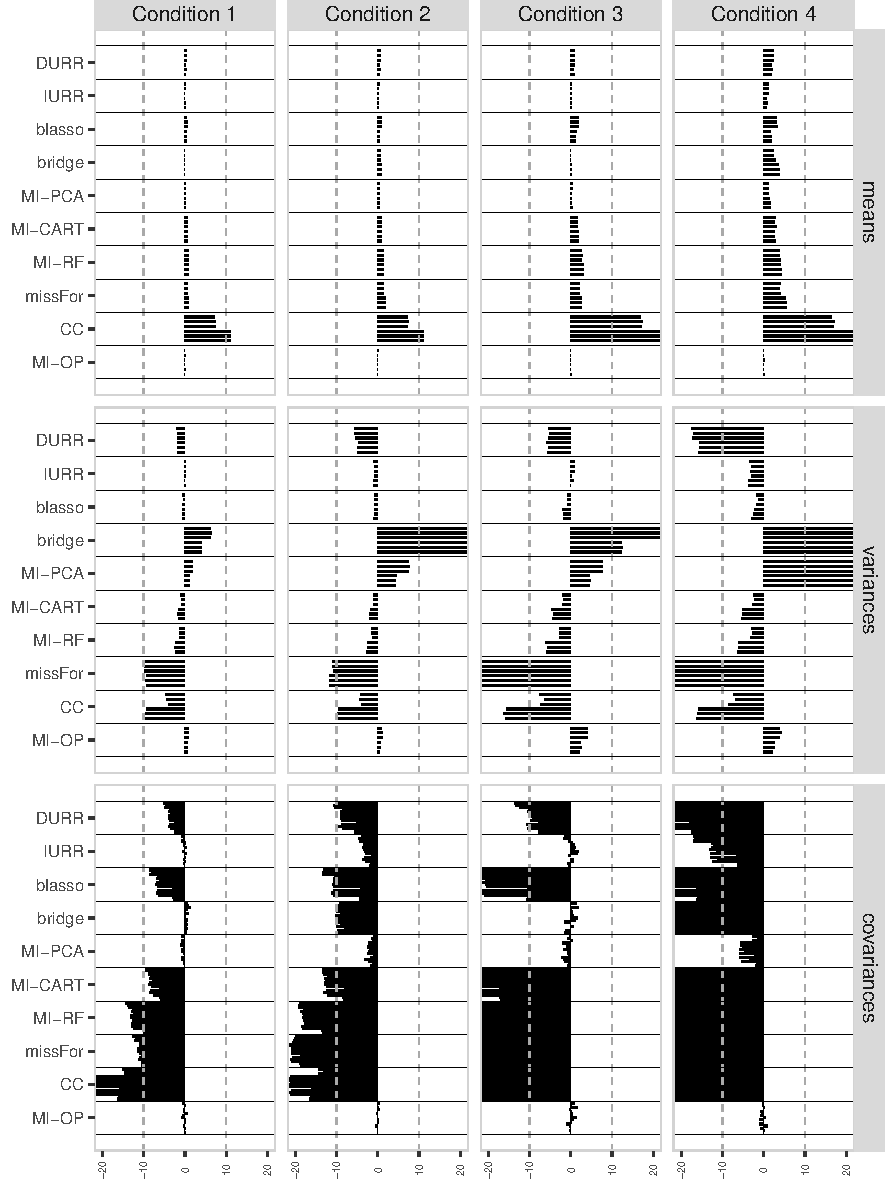
\includegraphics{../../output/graphs/exp1_bias.pdf}
\caption{Percent Relative Bias (PRB) for item means, variances, and covariances broken 
	down by method}
\label{fig:exp1bias}
\end{figure}

\begin{figure}
	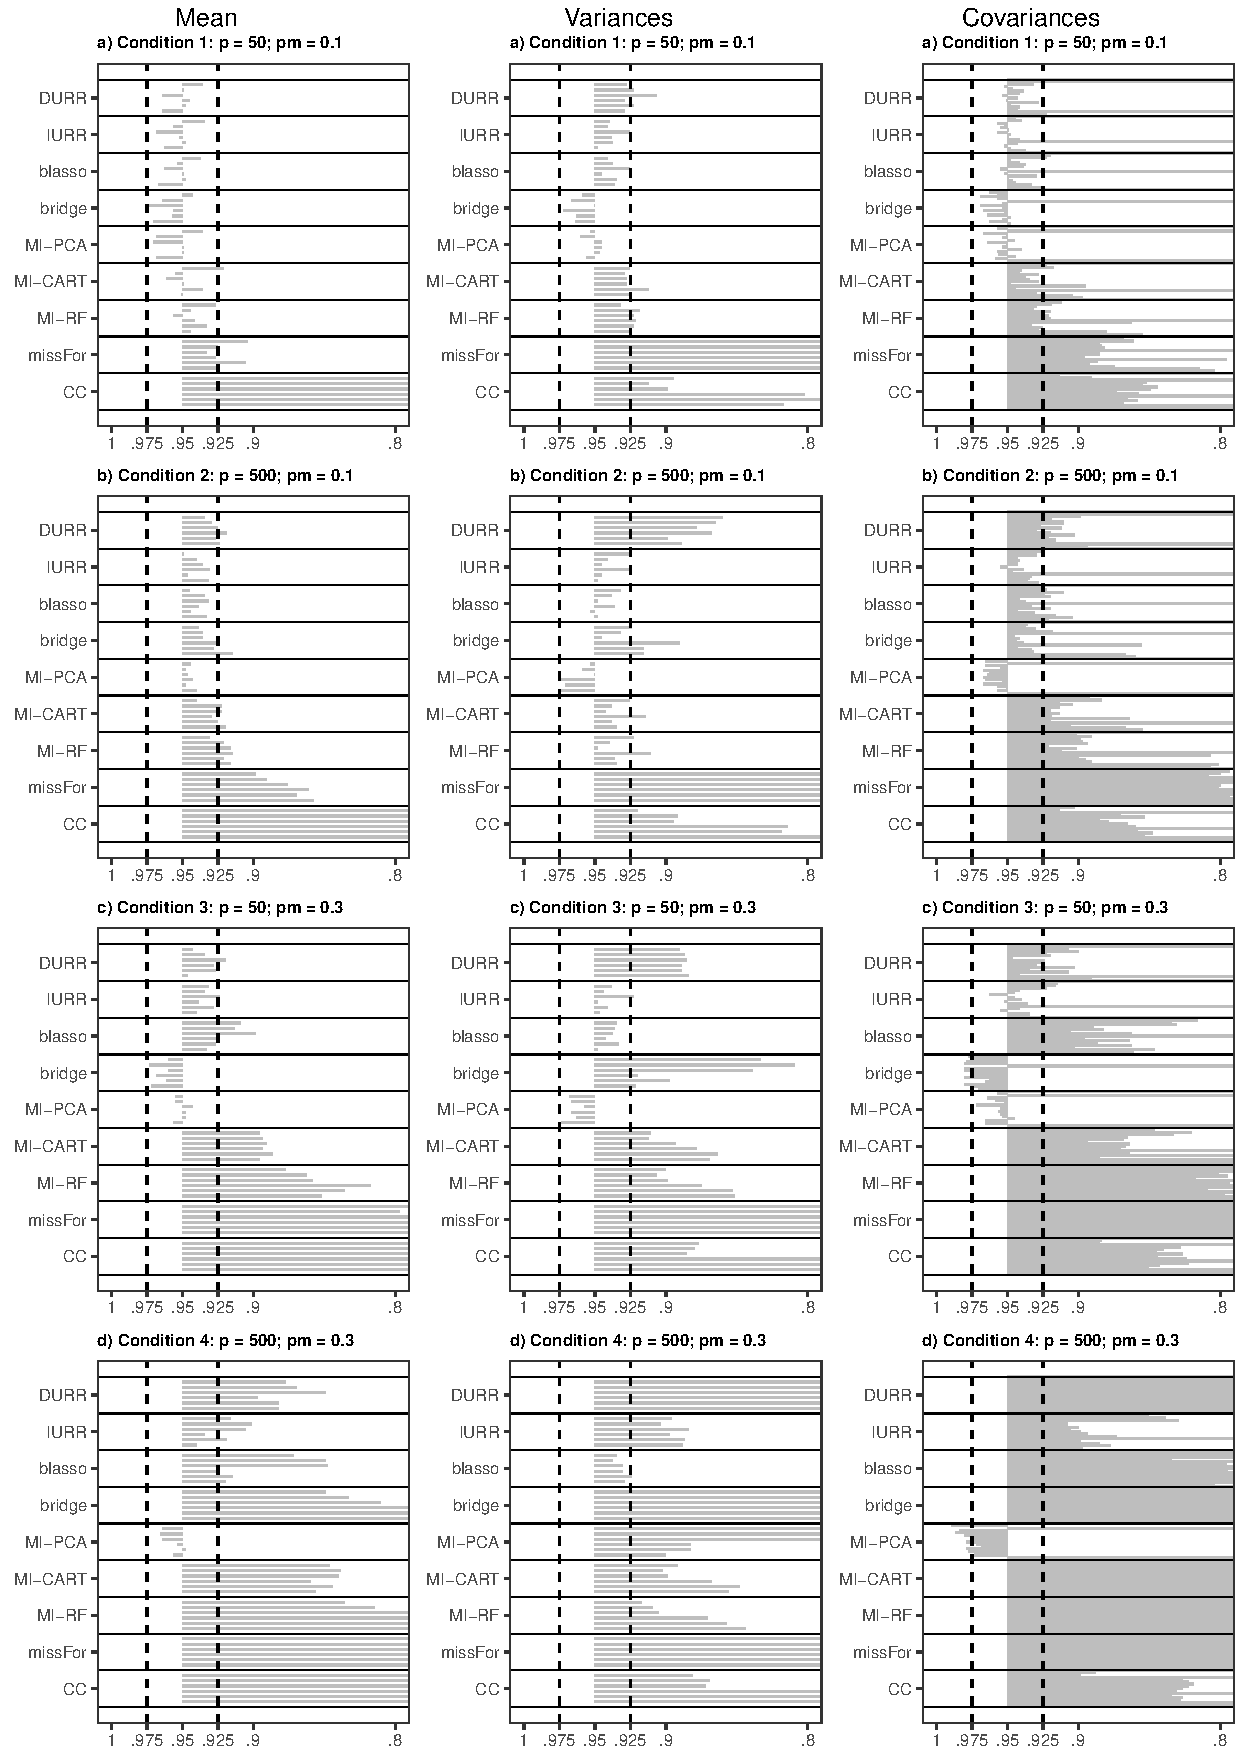
\includegraphics{../../output/graphs/exp1_CI.pdf}
\caption{Confidence Interval Coverage (CIC) for item means, variances, and covariances broken 
	down by method.}
\label{fig:exp1cir}
\end{figure}
	
\FloatBarrier % stops fig:exp1cir to leave its section

\subsubsection{Experiment 2}

\paragraph{Saturated Model}

	Results form the first experiments held mostly constant in experiment 2, indicating that the presence and 
	strength of a latent structure does not perturb the methods' relative performances.

	Figure \ref{fig:exp2bias} reports the bias of the saturated model parameter estimates for the first
	four conditions of experiment 2 (high factor loadings). 
	For both item variances and covariances PRB is reported, while for the item means we reported the SB. 
	Items were generated around a mean of 0 making the computation of PRB for this parameter meaningless.

	The least biased estimates for means and variances are obtained with IURR, in all conditions.
	Imputing missing values with the MI-PCA approach also grants low biases in all conditions.
	Bridge is also performing quite well with the exception of covariance estimates in condition 4.

	In agreement with what was found in experiment 1, the MI-PCA approach is the one resulting in the lowest
	bias for all covariance estimates in all conditions.
	Surprisingly, the bias for the item variances that afflicted MI-PCA in the multivariate-normal
	set up disappears when the latent structure is strong (factor loadings larger than .9).

	Figure \ref{fig:exp2cir} shows results for the confidence interval coverage in experiment 2.
	When factor loadings are high, we see that all multiple imputation methods lead to acceptable coverage 
	for means and variances, in the conditions with low proportion of missing values, no matter the 
	dimensionality of the data: in condition 1 and 3, for both item means and variances, confidence 
	intervals coverage is approximately within .93 and .97 for all methods.

	As the proportion of missing values increases we see a general deterioration in CIC performances, 
	with IURR and MI-PCA still showing the most contained deviations from the target value.
	Again, MI-PCA tends to include the true parameter values more than it should (over-coverage), 
	while most other methods show sings of under-coverage.

	Given the large positive biases obtained by all methods for the covariances of the observed items,
	it comes to no surprise that most methods lead to under-coverage of these parameters in all
	conditions in experiment 2. 
	MI-PCA is again the only exception providing acceptable coverage for all covariances.

	The same patterns can be seen in the conditions with lower factor loadings (see figures \ref{fig:exp2bias58} 
	and \ref{fig:exp2bias58} reported in appendix).
	However, in condition 8, the MI-PCA approach tends again to over-estimate the item variances (PRBs > 20\%)
	and it also leads to extreme under-coverage of this parameters.

\begin{figure}
	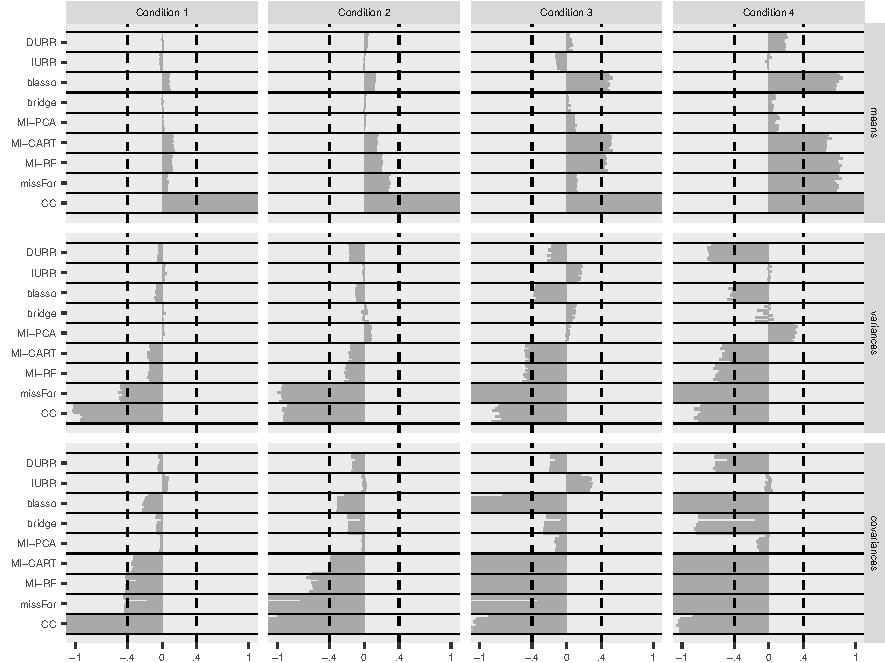
\includegraphics{../../output/graphs/exp2_semR_bias_sd_14.pdf}
\caption{Bias estimation for the means (SB), variances and covariances (PRB) for condition 1 to 4.}
\label{fig:exp2bias}
\end{figure}

\begin{figure}
	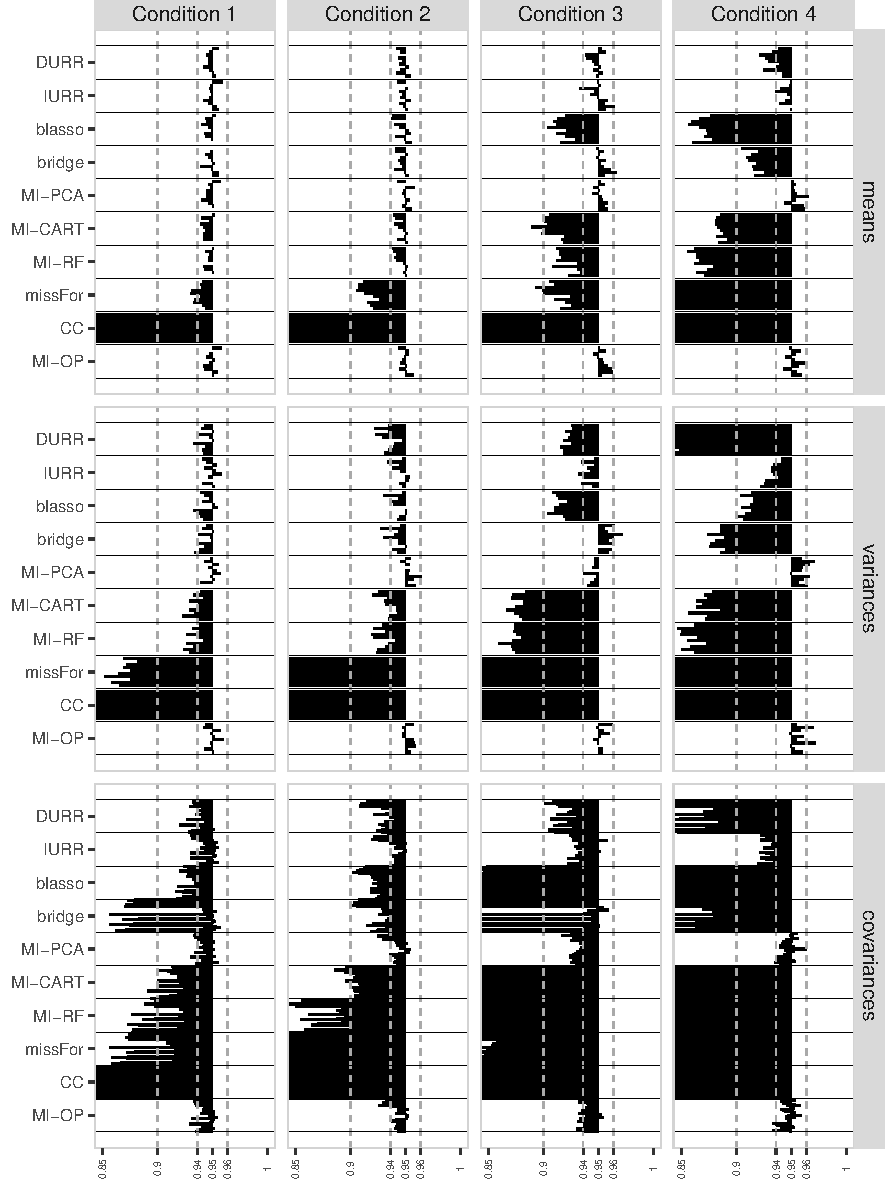
\includegraphics{../../output/graphs/exp2_semR_ci_14.pdf}
\caption{Confidence Interval Coverage (CIC) for the means, variances, and covariances for condition 1 to 4.}
\label{fig:exp2cir}
\end{figure}

\FloatBarrier % stops fig:exp2cir to leave its section

\paragraph{Confirmatory Factor Analysis}

	Figures \ref{fig:exp2fl14} shows the PRB values for all the factor loadings estimated by
	the Confirmatory Factor Analysis described above. 
	Most MI-Methods are able to provide acceptably low biased estimates for these parameters in 
	all conditions except the ones with both large proportion of missing values and high 
	dimensional input data matrix (condition 4).

	IURR and MI-PCA are again the two top performers giving virtually unbiased estimates
	of the factor loadings in all conditions.
	However, MI-PCA outperforms IURR when factor loadings are low, maintaining inconsequential 
	biases even when data is high-dimensional and the proportion of missing values is high.

\begin{figure}[h]
	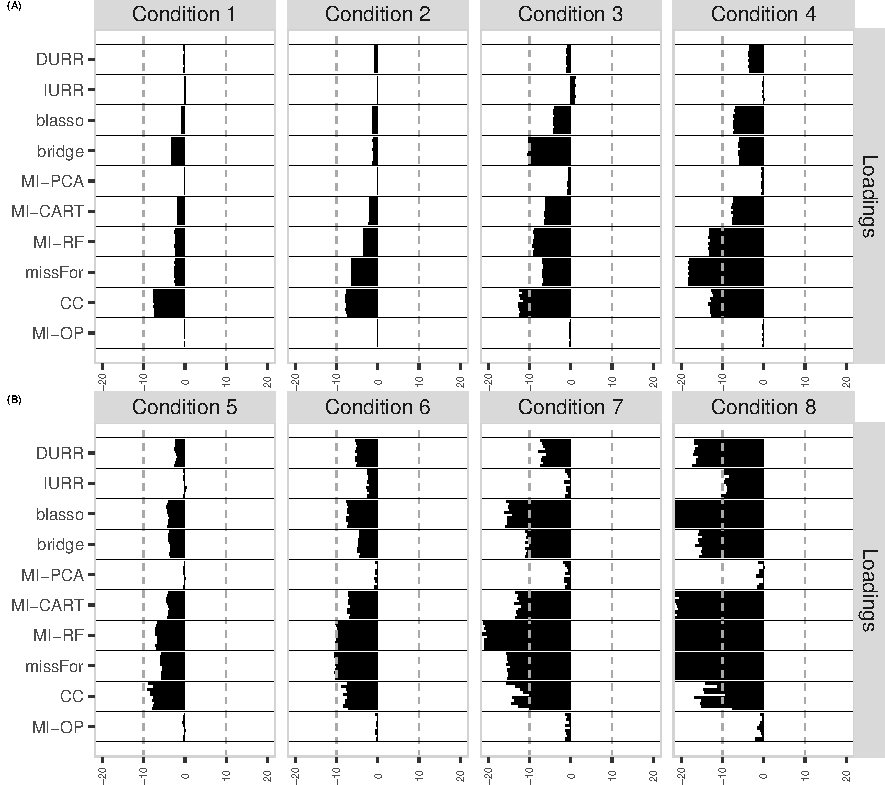
\includegraphics{../../output/graphs/exp2_CFA_lambda_BPR.pdf}
	\caption{Percent Relative Bias (PRB) for the factor loadings conditions 1 to 4 (panel A) 
		and conditions 5 to 8 (panel B).}
\label{fig:exp2fl14}
\end{figure}

\FloatBarrier % stops fig:exp2fl to leave its section



% Simulation Study 2

\maketitle
\section{Resampling Study}

To test the ecological validity of findings in experiment 1 and 2 we have also designed a
resampling study based on European Values Survey data.
By using data gathered for an actual survey, we can mostly observe whether the relative 
performances of the imputation methods change when they are deployed for real data research.
Variables in the EVS data are not generated artificially from continuously normal distributions 
but are discrete numerical items that are treated as such by researchers.

The resampling study follows a similar strategy to that used in the simulations. 
To assess the statistical validity of the different imputation methods we have repeated the 
following steps 1000 times ($R = 1000$):

\begin{itemize}
	\item Data generation - A bootstrap sample $\bm{X}^{*}$ was generated by sampling with replacement $n$ 
		observations from a pre-processed EVS data-matrix. 
		Part of the pre-processing step was some form of imputation used to obtain a pseudo-fully observed 
		input data matrix.
	\item Missing data imposition - Missing values were imposed on a given number of target variables
		in $\bm{X}^{*}$, according to some response model.
	\item Imputations - Each method described in section 2 to deal with missing values was used to impute
		NAs.
	\item Analysis - Two analysis models were fitted to the differently treated data.
		Parameters estimates pooled across the differently imputed datasets for the MI methods and
		stored along with the estimates obtained with single imputation methods and complete case 
		analysis.
\end{itemize}

	The average estimate, over the $R$ repetitions, obtained with the Gold Standard approach are considered 
	as "true" reference values of the parameters in the analysis models.
	The $R$ estimates obtained with all other methods are used to obtain performance measures for each imputation 
	method using the same criteria described for study 1 and 2 (see \ref{criteria}).

	The code to Run the simulation was written in the R statistical programming language (version 4.0.3). 
	The resampling study was run using a 2.6 GHz Intel Xeon(R) Gold 6126 processor, 523780 MB of Memory. The
	operating system was Windows Server 2012 R2.

	Computations were run in parallel across the available cores (between 30). Parallel computing 
	was implemented using the R package 'parallel' and to ensure replicability of the findings seeds were
	set using the method by \cite{lecuyer:2002} implemented in the R package 'rlecuyer'

\subsection{Methods}

\paragraph{Data preparation}
	EVS is a standardizes cross-sectional survey with a representative sample of more than 60,000 
	people, across more than 30 countries, interviewed via Web, post or face-to-face.
	For this study we have used the third pre-release of the 2017 wave of EVS data \citep{EVS:2017}.
	The original dataset contained 55,000 observations in 34 countries.

	We selected only the four European Founding Countries included in the data (France, Germany,
	Italy, and the Netherlands) and excluded all columns of the data that were either duplicated
	information (recoded versions of other variables), or linked to meta data (e.g. time of interview,
	mode of data collection). 
	All missing values were filled in with a run of a single imputation predictive mean matching (PMM) 
	which allowed us to obtain a pseudo fully-observed dataset. PMM was chosen for the task as it 
	is an effective, flexible imputation method that maintains the distributional characteristics of 
	the original data. 
	The full cleaning process is more systematically described in the appendix.

	At the end of this data cleaning process, we ended up with a fully-observed dataset
	of 8045 observations ($n$), across 4 countries, and 243 variables ($p$).

\paragraph{Analysis model(s)}

	To define plausible analysis models we have searched the EVS database for articles using
	such data looking for suitable analysis models on which to test the effectiveness of 
	the different imputation algorithm.
	We have defined two linear regression models of the form:
	\begin{center}
		\begin{equation} \label{eqn:lm}
			\bm{y} \sim \beta_0 + \bm{\beta_1} \bm{x}_1 + \bm{\beta}_{-1} \bm{X}_{-1}
		\end{equation}
	\end{center}

	In model 1, inspired by \cite{koneke:2014}, the dependent variable is a 10-point EVS item measuring euthanasia 
	acceptance ('Can this always be justified, never be justified, or something in between?'); the predictor 
	of interest a 4-point item measuring the self-reported importance of religion in one's life.
	A variety of covariates, such as measures of trust, education, and socio-economic status, were included in 
	$\bm{X}_{-1}$ as control variables.

	This model represents a plausible analysis a researcher would perform to test a theory regarding the 
	effect of religiosity on end-of-life treatments.

	In model 2, inspired by \cite{immerzeel:2015}, the dependent variable is an harmonized variable
	constructed by EVS to describe the respondents' tendency to vote on a 10-point left-to-right continuum; 
	the predictor of interest is a composite mean scale measuring respondents attitudes toward immigrants 
	and immigration ('nativist attitudes scale').
	Respondents expressed how much they agreed on a scale from 1 to 10, with the following statements: 
	'immigrants take jobs away from natives', 'immigrants increase crime problems', and 
	'immigrants are a strain on welfare system'.
	The control variables used included the usual socio-economic background information, the same measure of
	religiosity used in model 1, and some measures of political interest.

	A research might fit this model to their data and look at the regression coefficient of the nativist attitudes
	scale to test some theory regarding its effect on voting for right wing parties.

\paragraph{Missing data imposition}

	Missing data were imposed on 6 variables according to the same strategy as in \ref{subsub_missing}.
	The target variables we identified were the two dependent variables in models 1 and 2, religiosity (predictor
	in both models) and the three items making up the nativist attitudes scale (predictor in the second model).

	The response model form is the same as in \label{eqn:rm} and 3 variables were included in $\tilde{X}$: 
	age, education, and an item measuring trust in new people. 
	These are plausible variable that influence response tendencies in participants: 
	older people usually have higher item non-response rates than younger;
	so do lower educated compared to higher educated people; 
	people that have less trust in new people are assumed to withhold more information from the interviewer.

\paragraph{Conditions}
	There were only two conditions for the resampling study: low and high dimensional imputation.
	As the number of predictors in the data is fixed ($p = 250$), the dimensionality of the data is
	changed by defining different sizes for the sample taken from the pseudo-fully observed data.
	We chose only two values for $n$, namely $1000$ and $300$, corresponding to the low and high 
	dimensional condition.

\subsection{Results}
\subsubsection{Bias}

	\paragraph{PRB}
	Figure \ref{fig:exp4bias} reports the PRB for the regression coefficients of interest in model 1 and 2.
	Most of the MI methods result in negligible biases ($PRB < 10\%$) for both parameters in all conditions.
	The only two exceptions are bridge and MI-RF: the former is very competitive in condition (a), the low
	dimensional one, but leads to extreme bias in the high dimensional condition (b); the latter provides, 
	in all conditions, the highest PRB among the MI methods, it is consistently outperformed even by
	Complete Case analysis, and results in a 10\% PRB for the regression coefficient of nativist attitudes 
	in model 2.

	DURR and IURR are giving inconsequential biases for both parameters in all conditions, with PRBs that are
	often at least half in size as the ones obtain with the other methods.

	\paragraph{Euclidean Distance}
	Figure \ref{fig:exp4biased} reports the Euclidean Distance between the vector of estimated regression 
	coefficients for model 1 and 2.
	IURR and DURR yielded the vectors of parameters estimates that are closer to the vector of true values.
	The advantage in using these methods over others is stark for model 2 while it is less marked in model 1.
	While in the low dimensional condition, IURR does not seem to provide a lower bias than the other 
	methods, its relative performance improves as the dimensionality of the data increases.

	MI-PCA seems to struggle with bias for model 1, ranking last among the multiple imputation models.
	Nevertheless, it does provide a stark advantage compared to mean imputation and Complete Case analysis.

	Single imputation missForest is also able to provide a competitive vector of estimates, at least in model 2.

\begin{figure}
	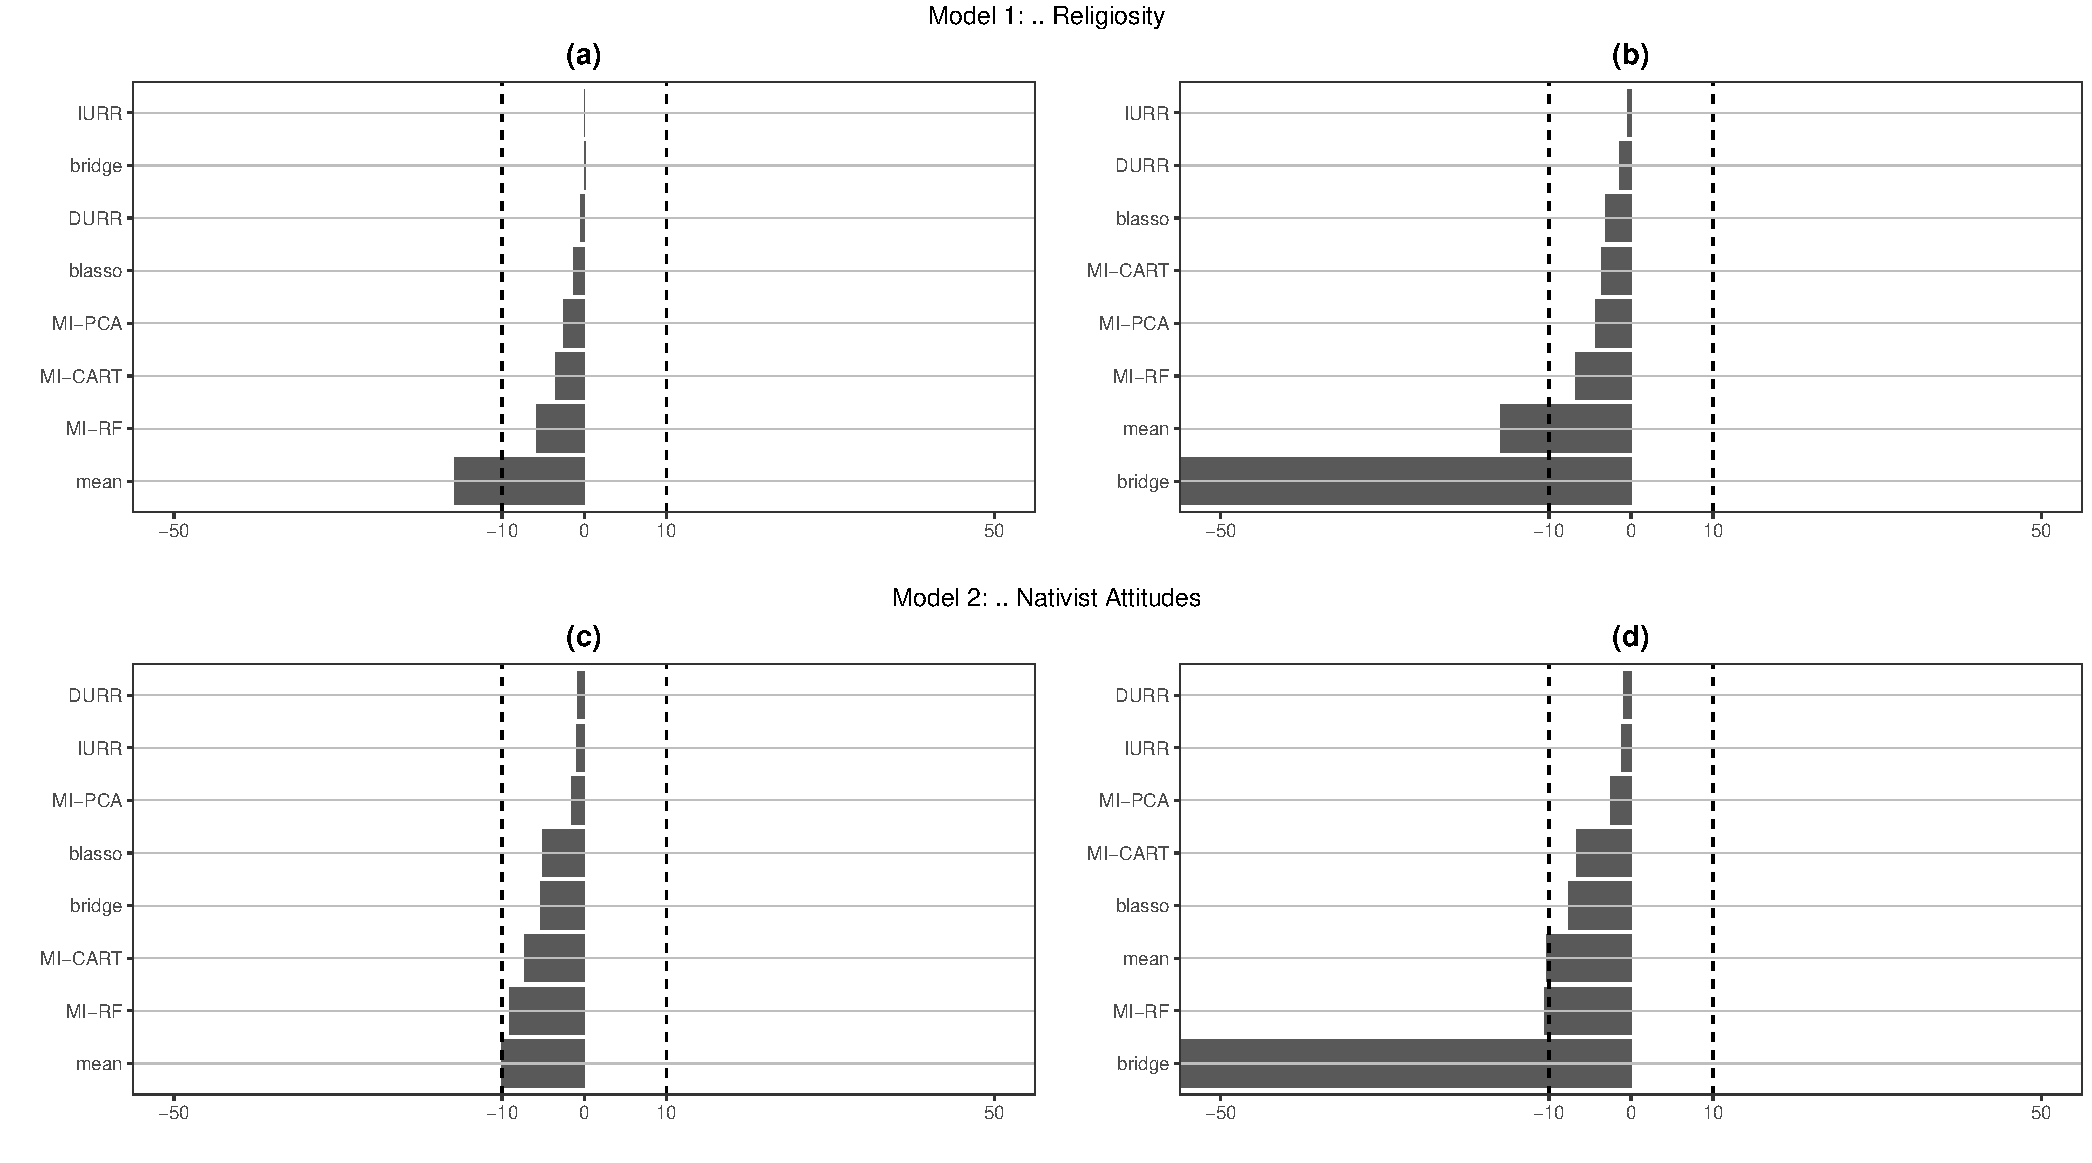
\includegraphics[width=\textwidth]{\pathFIG/exp4_imp_bias.pdf}
	\caption{Bias for single parameter of interest in the two different models}
	\label{fig:exp4bias}
\end{figure}

\begin{figure}
	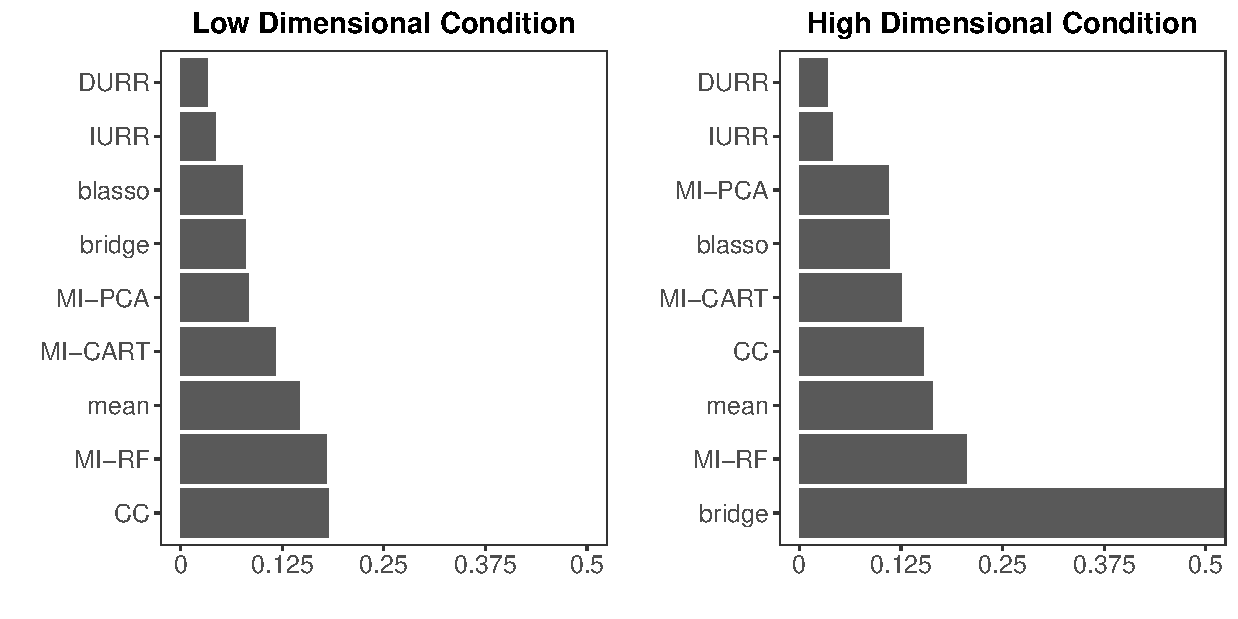
\includegraphics[width=\textwidth]{\pathFIG/exp4_ed_bias.pdf}
	\caption{Euclidean distance between the vector of estimated regression coefficients and
		the vector of their true value}
	\label{fig:exp4biased}
\end{figure}

\FloatBarrier

\subsubsection{Confidence Interval Coverage}

	\paragraph{Confidence Interval Coverage}
	Researchers interested in testing their theories with the inferential models described, will be interested
	in the confidence interval coverage of the estimates of interest.
	Figure \ref{fig:exp4ci} reports the CIR for the focal regression coefficient in the two models.

	Both IURR and DURR remain fairly competitive in terms of CIR, but the advantage they showed in terms of bias
	is not carried over to this criterion.
	Both MI-PCA and Blasso outperform IURR and DURR in almost all conditions, granting confidence intervals that 
	are noticeably closer to nominal coverage.
	
	\paragraph{Euclidean Distance}
	However, when looking at a more general pattern reported in \ref{fig:exp4cied}, IURR and DURR return to 
	the top of the leader-board, providing the closest vectors of Confidence Interval Coverages for model parameters 
	to nominal levels.

	\paragraph{Confidence Interval Width}
	Plot?

\begin{figure}
	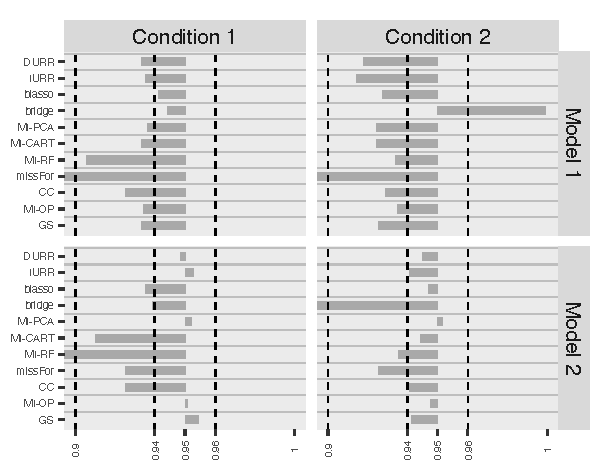
\includegraphics[width=\textwidth]{\pathFIG/exp4_imp_ci.pdf}
	\caption{Confidence Interval Coverage for single parameter of interest in the two 
		different models}
	\label{fig:exp4ci}
\end{figure}

\begin{figure}
	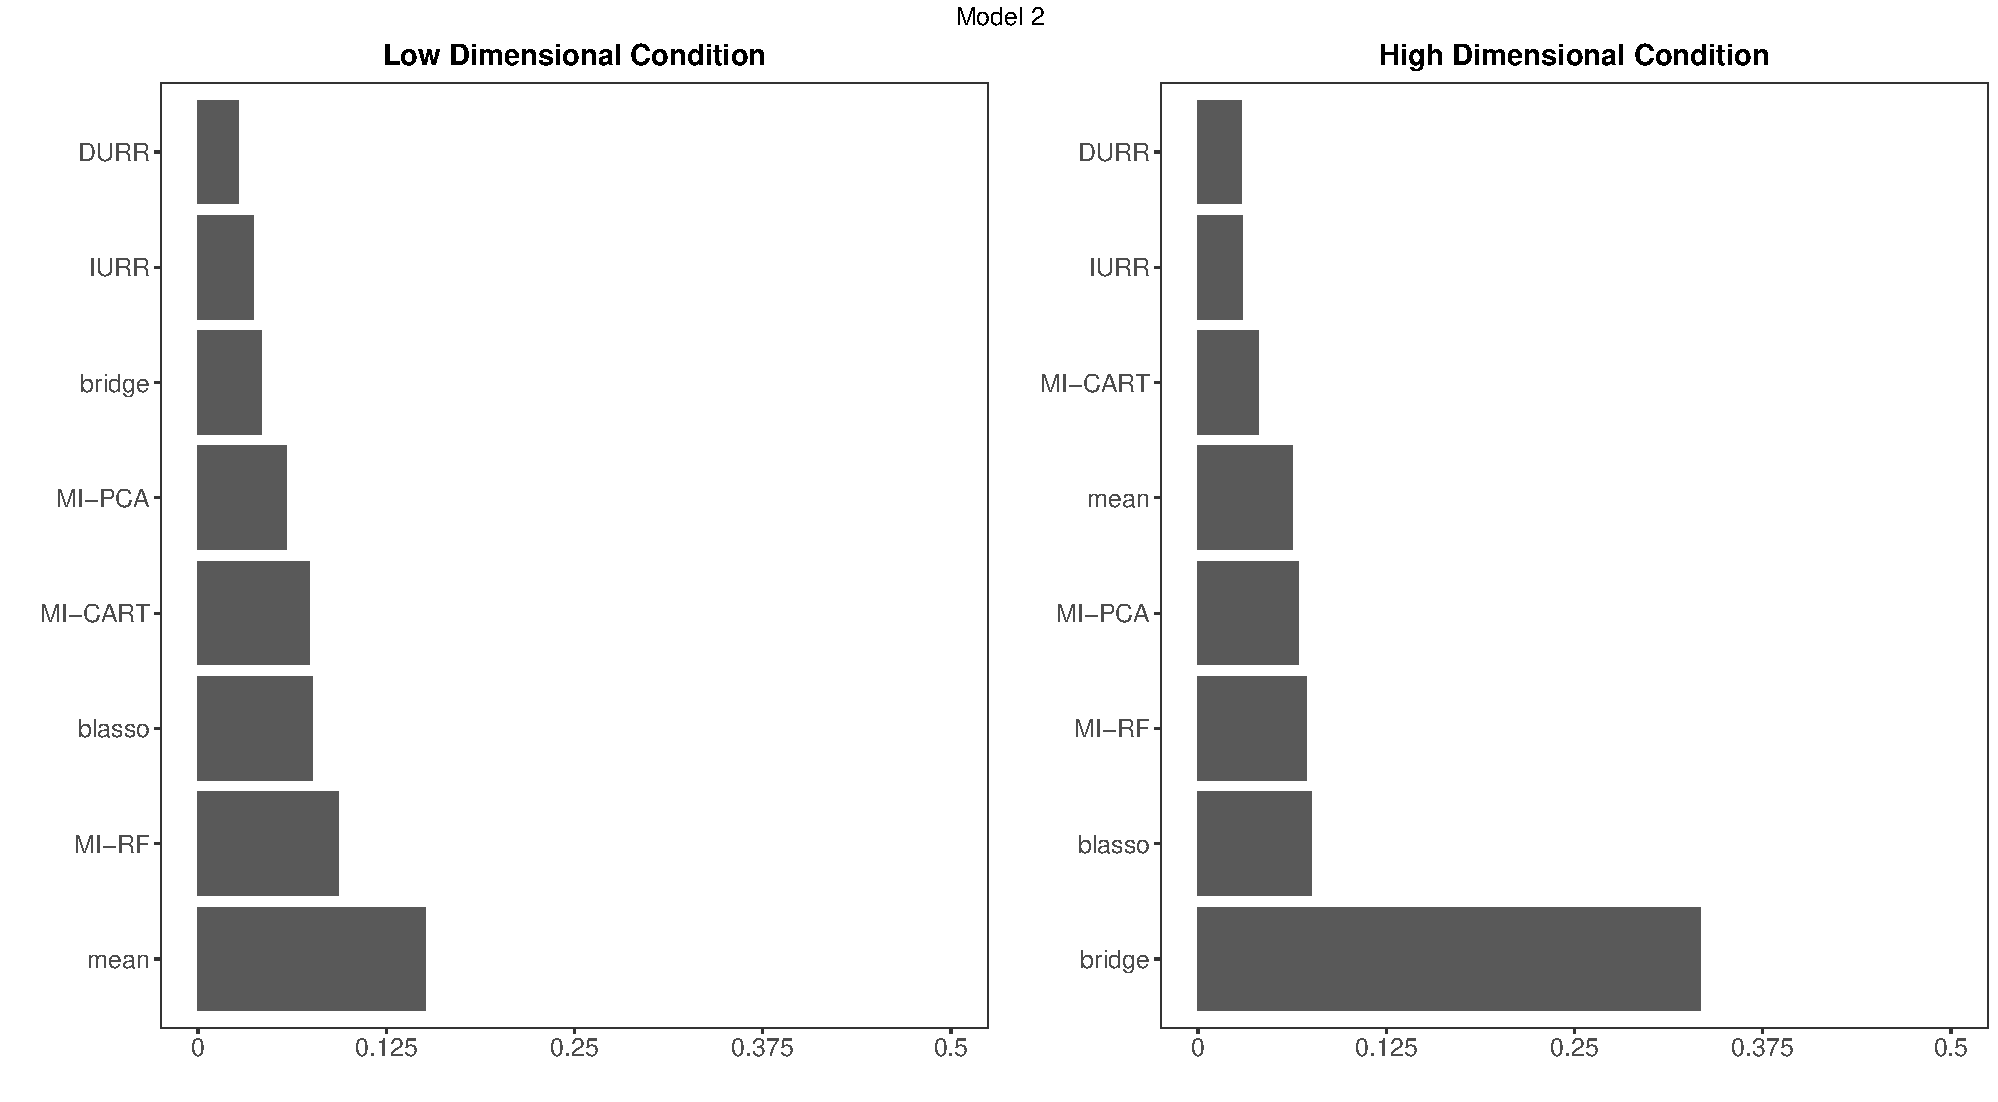
\includegraphics[width=\textwidth]{\pathFIG/exp4_ed_ci.pdf}
	\caption{Euclidean distance between the vector of confidence coverages and the vector of 
		nominal coverage}
	\label{fig:exp4cied}
\end{figure}

\begin{figure}
	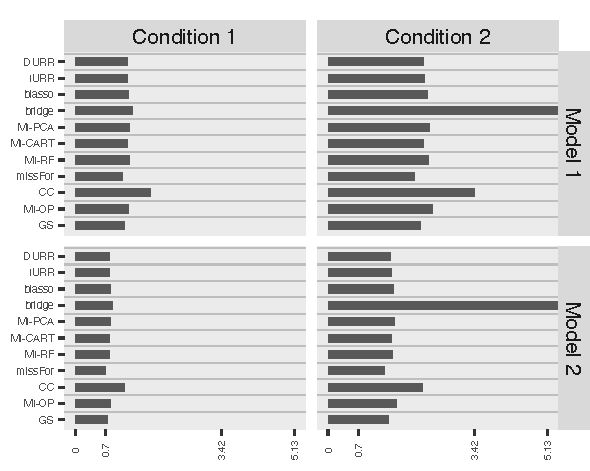
\includegraphics[width=\textwidth]{\pathFIG/exp4_imp_ciw.pdf}
	\caption{Confidence Interval Width for given parameter}
	\label{fig:exp4ciw}
\end{figure}

\FloatBarrier

\subsubsection{Imputation Time}

	Figure \ref{fig:exp4time} shows the average imputation time across the different methods.
	IURR and DURR are the most time consuming methods with imputation times above the hour, 
	in our low dimensional conditions, versus imputation times of a minute or less for MI-PCA and 
	Blasso imputation.
	In the high dimensional condition, the IURR and DURR are not as time-intensive, but still 
	require more then ten times the time of MI-PCA and blasso imputation.

\begin{figure}
	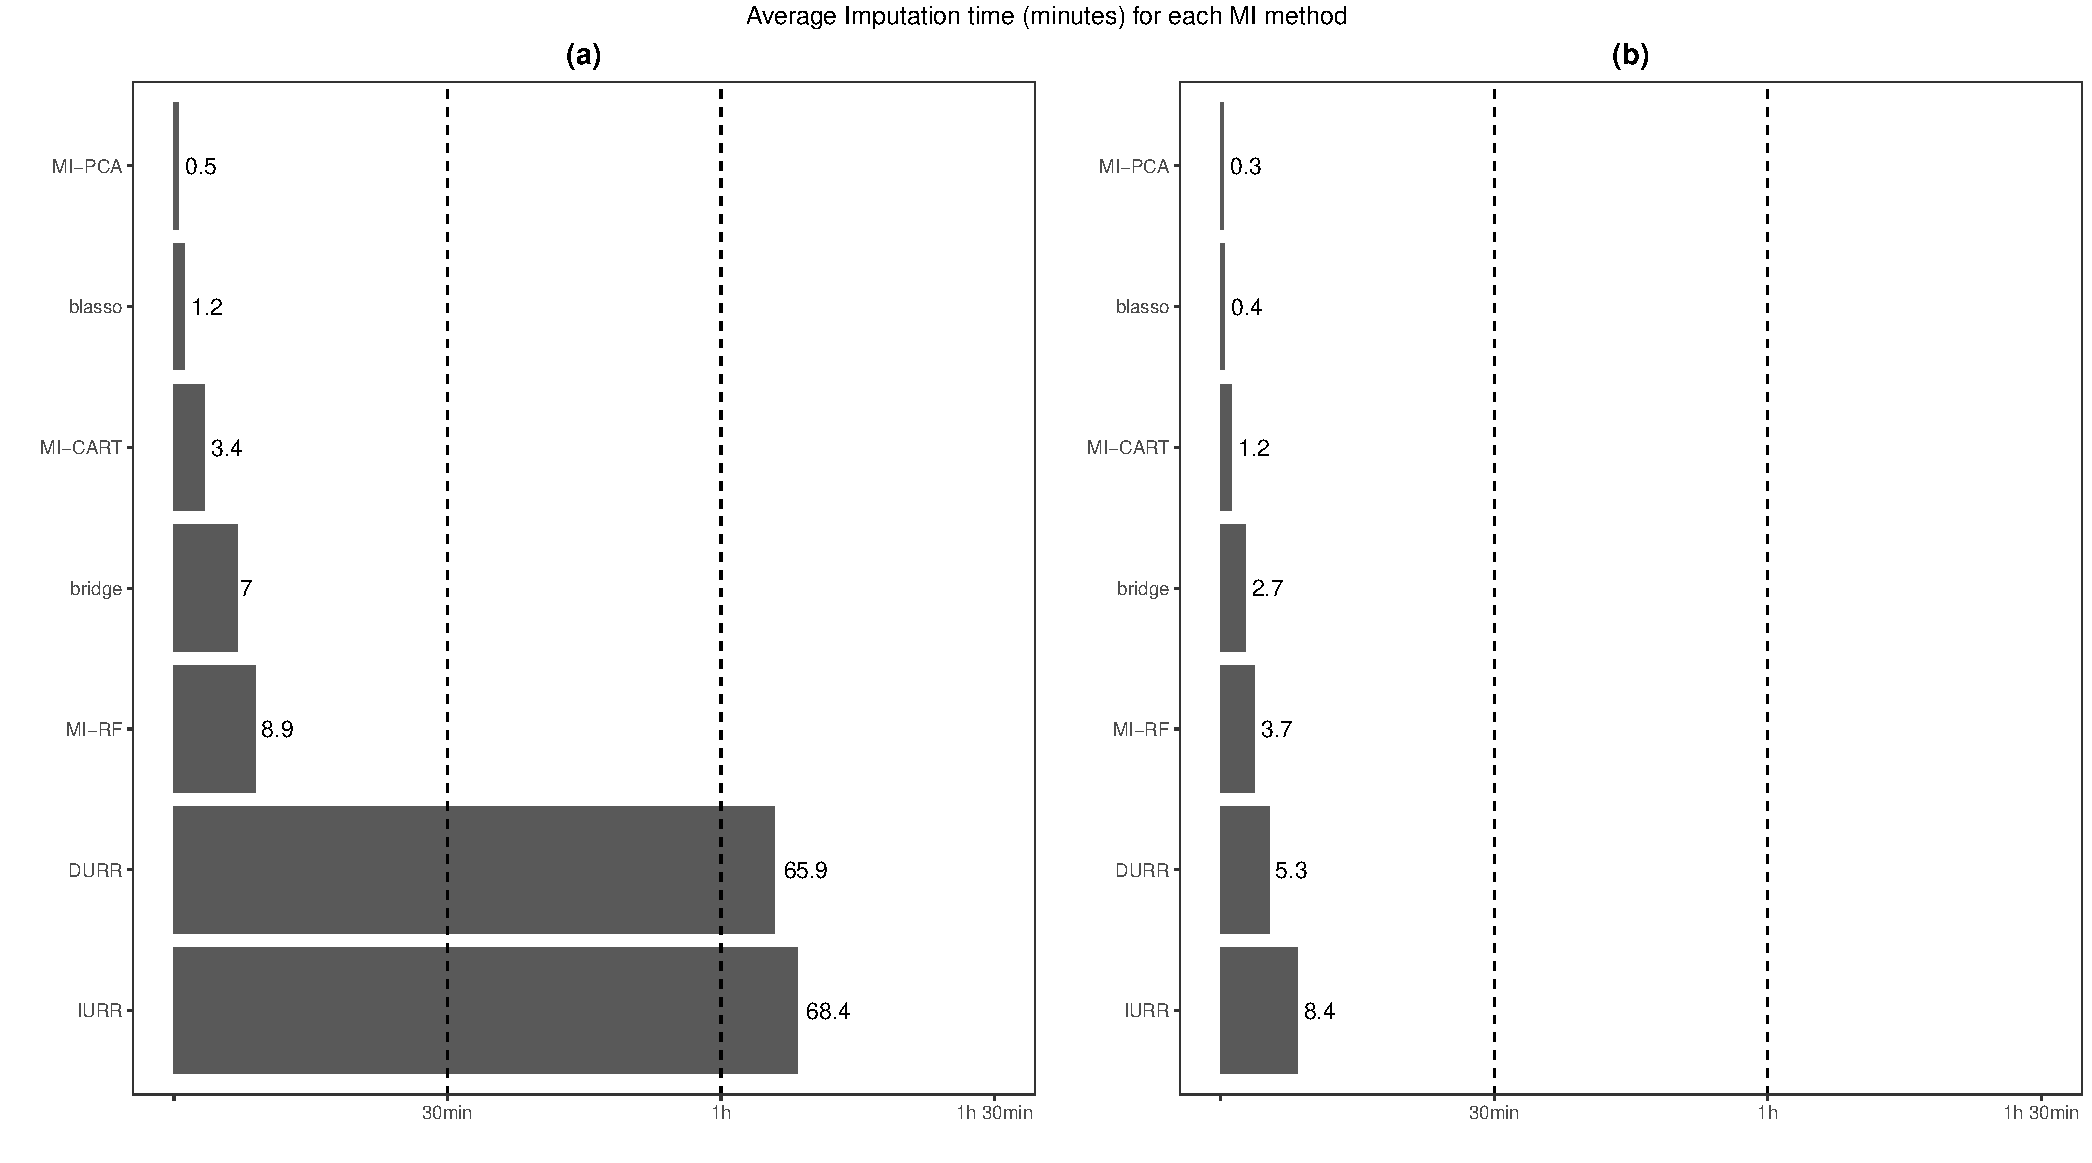
\includegraphics[width=\textwidth]{\pathFIG/exp4_time.pdf}
	\caption{Average imputation time for each method}
	\label{fig:exp4time}
\end{figure}

\FloatBarrier




% Resampling Study

\section{Discussion}

In what follows, the results obtained with the simulation and the resampling studies are discussed to provide
an overall picture of how the methods compare to each other.

\paragraph{IURR and DURR effective but time consuming}
	Overall, DURR and especially IURR showed great performances in all experiments according to all performance measures.
	However, using them requires a lot more imputation time than other well performing methods.
	For example, while both IURR and MI-PCA have weaknesses, overall, they showed similar performances for most parameters 
	and performance measures.
	However, MI-PCA obtained these results in a fraction of the time taken by IURR.

\paragraph{MI-PCA struggle with item variances}
	The bias for the item variances that afflicted MI-PCA in the multivariate-normal set up appears to be related to 
	the strength of the latent structure: when the latent structure is absent (experiment 1) or weak (experiment 2, 
	conditions 5 to 8, factor loadings between .5 and .6) item variances are biased, especially in the high-dimensional
	conditions; 
	when the latent structure is prominent (experiment 2, conditions 1 to 4), the variances are estimates with 
	negligible bias, even in the high-dimensional conditions.

	In general, MI-PCA tended to over-estimate (positive bias) the item variances while it was the only method
	with acceptable bias for the covariances.
	In other words, it seems that MI-PCA includes a lot of uncertainty regarding the imputed values, but it recovers 
	correctly the relationships between variables.

\paragraph{MI-PCA IURR trade off}
	Looking at the results from the simulations, it seems that the two most promising methods, IURR and MI-PCA, 
	show different weaknesses and strengths in terms of bias.
	The two simulations studies, showed that, in the high dimensional condition, MI-PCA struggles with correctly 
	recovering item variances but returns very lowly biased item covariances, while IURR shows exactly the opposite 
	behaviour.

	The resampling study showed that slightly more biased estimates of the parameters in model 1 and 2 are produced 
	using MI-PCA rather than IURR, while coverage rates and confidence interval widths did not substantively differ.
	This difference did not show when looking at the focal regression coefficients, where MI-PCA performed as well 
	as IURR, if not better.
	
	Overall, the simulation studies seemed to suggest that MI-PCA could recover more accurately the relationships
	between variables (less biased covariances) than IURR, while in the resampling study this conclusion was not
	supported to the same extent: when looking at bias and coverage rates for $\beta_{1,1}$ and $\beta_{1,2}$, MI-PCA 
	performed equally well or better than DURR and IURR, while looking at the overall measures of bias and coverages
	IURR and DURR outperformed MI-PCA.

\paragraph{Bridge inadequacy for high-dimensional set ups}
	In both the simulation and resampling study the use of a fixed ridge penalty within the imputation
	algorithm to facilitate the inversion of the observed data matrix lead to extreme bias in the high
	dimensional conditions.

\paragraph{Data Type Flexibility}
	Both IURR/DURR and MI-PCA allow for any type of data imputation with close to no effort.
	IURR and DURR have already been discussed for categorical data imputation, and MI-PCA can be performed
	with any standard imputation model for categorical data.
	The use of Bayesian Lasso however as yet to be developed for multi-categorical imputation target 
	variables.



% Discussion

\section{Discussion}

	The inclusion of high-dimensional prediction techniques within the MICE framework has the potential
	to simplify the use of MI for social scientist.
	We studied bias and coverage of parameter estimates after imputation by seven high-dimensional data 
	MI methods.
	Although extensive simulation studies had already been carried out by the researchers proposing these methods, 
	no comparison study had been developed to assess their relative performance.
	Our research fills this gap and provides initial insights into applying such methods in social scientific research.
	In this section, we discuss the overall performance of the methods and we give recommendations for social scientists 
	facing high-dimensional data imputation problems.

\paragraph{Methods that do not work well}

	We found that bridge is inadequate to deal with high-dimensional data imputation problems.
	In both the simulation and the resampling study the use of a fixed ridge penalty within the imputation
	algorithm manifested the same undesirable performance.
	The method worked well when many predictors were included in the imputation model, but the imputation
	task remained low dimensional.
	However, bridge led to extreme bias and unacceptable confidence interval coverage in all the high 
	dimensional conditions.

	We have also confirmed that missForest, the high-dimensional data SI method, leads to low estimation 
	bias, but results in severe confidence interval under-coverage of the true parameter values.
	Under-coverage coupled with unbiased estimates indicates that too little uncertainty is incorporated in 
	the imputation procedure, which is to be expected from a single imputation approach.
	As a result, missForest should be avoided by social scientists with the goal of drawing inferential 
	conclusions from their data analysis.

\paragraph{Methods that work best}

	IURR and MI-PCA were the two strongest performers.
	IURR excelled with the smallest estimation bias for item means, variances and regression coefficients.
	The method also produced small deviations from nominal coverage rates for these parameters.
	Furthermore, the large covariance estimation bias introduced by IURR in the high-dim-high-pm conditions
	only slightly exceeded the 10\% threshold and the CI coverage was just around 0.9.
	Comparatively, most of the other MI methods resulted in covariance PRBs larger than 20\%, and CICs 
	well below 0.9.

	Compared to regular low dimensional MI, IURR does not require the imputer to make choices regarding which variables
	are relevant for the imputation procedure.
	The only additional decision required of the imputer is the number of folds for the cross-validation of lasso 
	penalty.
	As a result, IURR is easy to specify and an extremely appealing method for imputation of large social scientific 
	datasets.
	However, IURR is a relatively computationally intensive.
	If the number of variables with missing values is large, IURR might result in prohibitive imputation time.
	In such a scenario, a researcher might prefer to address imputation with the MI-PCA method.

	MI-PCA showed low bias and good coverage for both item means and covariances in experiments 1 and 2.
	Although it exhibited large bias of the item variances, the relationships between variables with missing values 
	were always correctly estimated.
	It was the only method resulting in low bias and close-to-nominal CI coverage of the true covariance values,
	even in the high-dimensional conditions.
	Furthermore, it produced the lowest bias for the latent factor loadings.	
	MI-PCA also resulted in low bias and CIC close to nominal rates for the focal regression coefficient
	in Experiment 3.
	Finally, when the CICs obtained with MI-PCA deviated significantly from nominal rates, they over-covered.
	This tendency is less worrisome than under-coverage as it leads to conservative, rather than liberal, 
	inferential conclusions.
	As a result, this method is excellent approach for data analysts interested in testing theories on 
	large social scientific datasets with missing values.

\paragraph{Methods with mixed results}
	DURR produced low bias and good CI coverage for item means, variances, and regression coefficients.
	However, compared to IURR, it suffered from greater performance deterioration when applied to 
	high-dimensional data. 
	As a result, our results suggest that DURR should not be preferred to IURR.

	There was little difference in performance between the use of CART and Random Forests as 
	building blocks of the MICE algorithm.
	In line with what \cite{dooveEtAl:2014} found, when a difference was noticeable, it was in favor of the use 
	of the simpler CART.
	Both MI-CART and MI-RF produced large covariance bias in experiments 1 and 2.
	Although, bias for means, variances, and regression coefficients was acceptable, it was usually larger 
	than that obtained by other MI methods.
	Furthermore, in terms of CI coverage, they showed significant large under-coverage of most parameters in 
	the high-dim-high-pm conditions.
	Although the non-parametric nature of these approaches elegantly avoids over-parametrization of imputation models,
	these methods are outperformed by IURR and MI-PCA.

	Blasso resulted in low item means and variances bias, even in the high-dimensional conditions.
	While the covariance bias was large in experiments 1 and 2, blasso performed well in the resampling study, 
	where the overall biasing performance was similar to that of MI-OP.
	In terms of confidence interval coverage, blasso showed poor performance resulting in either CI 
	under-coverage or CI over-coverage of true parameter values in almost all high-dimensional conditions.
	Furthermore, blasso did not fair particularly well in the recovery of the latent structure in our second 
	experiment.
	Its factor loading PRBs were the highest among the MI methods.

	Theses mixed performances of blasso are also accompanied by a few obstacles to its application for social 
	scientific research.
	Using \cite{hans:2010}'s Bayesian Lasso requires the specification of 6 hyper-parameters, which 
	introduces more researcher degrees of freedom and demands a strong grasp of Bayesian statistics.
	Furthermore, the method has not currently been developed for multi-categorical data imputation,
	a common task in the social sciences.
	As a result, blasso is not recommended for imputation of large social scientific datasets.


% Conclusions

\section{Limitations and future directions}

	The present work was aimed at comparing current implementations of existing imputation methods.
	As a result, the scope of the simulation and resampling studies was limited by the current development state of 
	the different methods.
	For example, DURR, IURR, and MI-PCA allow imputation of any type of data:
	DURR and IURR have been developed for categorical data imputation \citep{dengEtAl:2016},
	and MI-PCA can be performed with any standard imputation model for categorical data.
	However, blasso has not been formally developed for imputing multi-categorical variables yet. This limitation of blasso forced us to work with missing values on variables that are either continuous, or usually 
	considered as such in practice (e.g., Likert-type scales).
	To maintain a fair comparison with blasso, all methods were implemented with the assumption that the imputed 
	variables are continuous and normally distributed.
	However, IURR, DURR and MI-PCA could have performed differently in the resampling study if we had used their
	ordinal data implementations.

	Another limitation of this study is the assumption of a linear missing data mechanism.
	In real social scientific data, the response mechanism might be nonlinear, a condition that could require
	including transformations of the raw variables (e.g., interactions, polynomial terms) in the imputation models.
	Non-linear response models were not part of the scope of this project. 
	However, all of the high-dimensional imputation methods considered have the potential to account for more complex response mechanisms.

	Finally, these results only apply to the specific implementations of the algorithms we used. 
	Many of the methods discussed could have been implemented differently.
	\cite{zhaoLong:2016} proposed versions of IURR and DURR using the elastic net penalty \citep{zouHastie:2005} and 
	the adaptive lasso \citep{zou:2006} instead of the lasso penalty.
	Although no substantial performance differences between penalty specifications emerged 
	from the work of \cite{zhaoLong:2016} or \cite{dengEtAl:2016}, we must acknowledge that we did not investigate the impact of different types of
	regularization in the present study. 

	MI-PCA requires making a decision on the number of components to extract from the auxiliary 
	variables.
	In this study, we decided to retain the first components that explained 50\% of the total variance in the 
	auxiliary variables.
	However, this decision was arbitrary. 
	We plan on assessing its effect on the imputation accuracy as part of a project to 
	expand and improve the use of principal components within the MICE framework.

	As for blasso, we have not investigated the sensitivity of the results to different hyper-parameters choices.
	Furthermore, alternative implementations of Bayesian Lasso could be used within a MICE framework.
	In particular, the well-known Bayesian Lasso proposed by \cite{parkCasella:2008} is a viable option.

	We could have also implemented the random forests differently.
	We decided to use the \cite{dooveEtAl:2014} version which is supported in the popular 
	R package \emph{mice}.
	However, \cite{shahEtAl:2014} independently developed another implementation of random forests
	within the MICE algorithm, which was available in the now archived R package CALIBERrfimpute
	\citep{CALIBERrfimpute}.
	We are not aware of any evidence or theoretical reason to expect differences between the two implementations, 
	but we did not verify this empirically.



% Bibliography
\bibliographystyle{apacite} 

\bibliography{
	\pathBIB/missingData/bibtex/papers,
	\pathBIB/missingData/bibtex/books,
	\pathBIB/missingData/bibtex/software,
	\pathBIB/bayesStats/bibtex/papers,
	\pathBIB/programming/bibtex/papers,
	\pathBIB/survey/bibtex/data,
	\pathBIB/survey/bibtex/studies,
	\pathBIB/statsLearn/bibtex/books,	
	\pathBIB/statsLearn/bibtex/papers,
	\pathBIB/statsLearn/bibtex/software
	}

\end{document}
